% concatenated from ERI.tex
\documentclass[11pt]{article}
\usepackage[utf8]{inputenc}
\usepackage[T1]{fontenc}
\usepackage[english]{babel}
\usepackage{amsthm,amsmath,amssymb}
\usepackage{geometry}
\geometry{margin=1in}
\usepackage{enumitem}
\usepackage{microtype}
\usepackage{xcolor}
\usepackage{url}
\usepackage[colorlinks=true,linkcolor=blue!70!black,citecolor=green!50!black,
            urlcolor=blue!60!black]{hyperref}
\usepackage{tikz}
\usetikzlibrary{arrows.meta,positioning}

\newtheorem{theorem}{Theorem}[section]
\newtheorem{lemma}[theorem]{Lemma}
\newtheorem{proposition}[theorem]{Proposition}
\newtheorem{corollary}[theorem]{Corollary}
\newtheorem{fact}[theorem]{Fact}
\theoremstyle{definition}
\newtheorem{definition}[theorem]{Definition}
\theoremstyle{remark}
\newtheorem{remark}[theorem]{Remark}
\newtheorem{example}[theorem]{Example}
\newtheorem{convention}[theorem]{Convention}
\newtheorem{openproblem}[theorem]{Open Problem}

\title{The Extended Real Line with Reentry:\\
Separating US from KC in the Clontz Hierarchy}
\author{Dami\'{a}n Rafael Lattenero\\[4pt]
\small\texttt{damian.lattenero@gmail.com}}
\date{March 2026}

\begin{document}
\maketitle

\begin{abstract}
We construct the \emph{Extended Real Line with Reentry} (ERI):
identify $\{-\infty, 0, +\infty\}$ to a single point $\ast$ in
$\overline{\mathbb{R}}$, and require every neighborhood of $\ast$ to
have dense preimage.
The resulting space is compact, path-connected, and sober; it is
$T_1$ and US (uniquely sequential), but not weakly Hausdorff, not
KC, and not Hausdorff.  In the refined hierarchy of
Clontz~\cite{bib:clontz} it sits at the $k_2$-Hausdorff level.
A search of pi-Base~\cite{bib:pibase} for compact US-not-KC spaces
returns three entries---$\mathbb{Q}^{\ast} \times \mathbb{Q}^{\ast}$,
$\omega_1{+}1$ with doubled endpoint (S37), and the one-point
compactification of the Arens--Fort space (S165)---all totally
disconnected.  ERI is the first compact path-connected example.

The same density condition on a general compact Hausdorff base
without isolated points defines a \emph{Filter-Modified Quotient}
(FMQ).  We prove that the density modifier $\mathcal{D}_Y$ is the
least restrictive admissible modifier preserving US, and that the
hierarchy level $k_2\mathrm{H}$-not-$\mathrm{wH}$ is invariant under
infinite closed nowhere-dense collapse sets, iteration of the
construction, and arbitrary products.  The only remaining direction
toward a US-not-$k_2\mathrm{H}$ level runs through non-first-countable
base spaces.
\end{abstract}

\smallskip
\noindent\textbf{MSC 2020:} 54A20, 54B15, 54D10, 54D25, 54D30, 54D55, 54G20.\quad
\textbf{Keywords:} US space, KC space, filter-modified quotient,
admissible modifier, density condition, Wilansky hierarchy,
$k_2$-Hausdorff, tightness, sobriety, infinite collapse set,
iterated quotient.

\tableofcontents

% =================================================================
\section{Introduction}\label{sec:intro}
% =================================================================

The study of separation axioms strictly between $T_1$ and $T_2$ was
initiated by Wilansky~\cite{bib:wilansky}.

\begin{definition}[Wilansky~\cite{bib:wilansky}]\label{def:USKC}
A space $X$ is a \emph{US-space} (uniquely sequential) if every convergent
sequence in $X$ has a unique limit, and a \emph{KC-space} (kompacts
closed) if every compact subset of $X$ is closed.
\end{definition}

The implications $T_2 \Rightarrow \mathrm{KC} \Rightarrow \mathrm{US}
\Rightarrow T_1$ are all strict~\cite{bib:wilansky,bib:alas}.
A refined hierarchy developed by Clontz~\cite{bib:clontz}, with
intermediate axioms drawn from the $k$-space and homotopical literature,
is
\begin{equation}\label{eq:clontz}
T_2 \;\Rightarrow\; k_1\mathrm{H} \;\Rightarrow\; \mathrm{KC}
\;\Rightarrow\; \mathrm{wH} \;\Rightarrow\; k_2\mathrm{H}
\;\Rightarrow\; \mathrm{US} \;\Rightarrow\; T_1,
\end{equation}
where a space is \emph{weakly Hausdorff} (wH) if every continuous image
of a compact Hausdorff space is closed, and \emph{$k_2$-Hausdorff}
($k_2$H) if for every continuous $f\colon K \to X$ with $K$ compact
Hausdorff the kernel $\{(a,b) \in K \times K : f(a) = f(b)\}$ is
closed~\cite{bib:clontzwilliams}.
The role of first-countability is classical:

\begin{fact}[see e.g.\ {\cite[p.~60]{bib:goreham}}]\label{fact:firstUS}
A first-countable space is Hausdorff if and only if it is US.
\end{fact}

The strict implications in~\eqref{eq:clontz} therefore collapse in
the first-countable setting, so any counterexample to
$\mathrm{US} \Rightarrow \mathrm{KC}$ has to fail first-countability at
some point.

The author is unaware of any compact path-connected space in the
literature that separates US from KC.
A search of pi-Base~\cite{bib:pibase}\footnote{Space IDs (S$n$)
throughout this paper refer to entries in the pi-Base community
database~\cite{bib:pibase}.} for compact US-not-KC spaces returns
three entries: the product $\mathbb{Q}^{\ast} \times \mathbb{Q}^{\ast}$,
the ordinal $\omega_1{+}1$ with doubled endpoint (S37), and the
one-point compactification of the Arens--Fort space
(S165)~\cite{bib:clontz}.
All three are totally disconnected.
Van~Douwen's anti-Hausdorff Fr\'{e}chet--Urysohn
space~\cite{bib:vandouwen} is compact and US, but it was built from a
MAD family and is KC by K\"{u}nzi--van der Zypen~\cite{bib:kunzi}.
The line with two origins is $T_1$ and first-countable, and there the
sequence $1/n$ has two limits, so US fails.

We construct such a space.
The \emph{Extended Real Line with Reentry} (ERI) is obtained from
$\overline{\mathbb{R}} = [-\infty, +\infty]$ by identifying
$\{-\infty, 0, +\infty\}$ to a single point $\ast$; the topology is
the coarsening of the standard quotient in which every neighborhood
of $\ast$ is required to have dense preimage.
ERI is compact, path-connected, and sober.
It is $T_1$ and US, and it is $k_2$-Hausdorff; it is not weakly
Hausdorff, not KC, and not Hausdorff.
The failure of first-countability at $\ast$ is forced by
Fact~\ref{fact:firstUS}, and $\ast$ is the only point at which ERI
fails to be first-countable.
At $\ast$ the tightness is $\aleph_0$ while the character is at least
$\aleph_1$, so ERI is an example of countable tightness without
sequentiality.

We now generalize the construction.
For any compact Hausdorff $Y$ without isolated points and any finite
nonempty $A \subseteq Y$, an admissible collection
$\mathcal{F} \subseteq \mathcal{P}(Y)$---a ``filter-like'' family
stable under supersets and suitable intersections---determines a
quotient topology on $Y/A$ by declaring an open set containing the
collapsed point open iff its preimage lies in $\mathcal{F}$.
We call the resulting space a \emph{Filter-Modified Quotient} (FMQ).
ERI is the FMQ in which $Y = \overline{\mathbb{R}}$, $A = \{-\infty,
0, +\infty\}$, and $\mathcal{F}$ is the collection $\mathcal{D}_Y$ of
dense subsets.
We show that the density modifier $\mathcal{D}_Y$ is the least
restrictive admissible modifier for which the quotient is US
(Theorem~\ref{thm:optimality}), and that the resulting hierarchy
level $k_2\mathrm{H}$-not-$\mathrm{wH}$ is stable under enlarging
$A$ to any closed nowhere-dense set, under iterating the
construction, and under products.
The only parameter we have not ruled out as a route to a higher
hierarchy level is first-countability of the base: the candidate is
$Y = \beta\mathbb{N} \setminus \mathbb{N}$, and the question is open.

The paper is arranged as follows.
Section~\ref{sec:construction} defines ERI and its basic separation,
connectedness, and dimensional properties.
Section~\ref{sec:countseq} develops the sequential theory and places
ERI in the Wilansky hierarchy.
Section~\ref{sec:k2H} proves the $k_2$-Hausdorff property and
compares ERI with the three known compact US-not-KC examples.
The FMQ framework is introduced in Section~\ref{sec:fmq}, the
modifier spectrum and the optimality theorem in
Section~\ref{sec:modifiers}, and the extended-rigidity results
together with further examples in Section~\ref{sec:extended}.
Open problems are collected in Section~\ref{sec:open}.

% =================================================================
\section{The ERI Space}\label{sec:construction}
% =================================================================

\subsection{Definition and notation}

\begin{definition}[ERI space]\label{def:ERI}
Let $\overline{\mathbb{R}} = [-\infty,+\infty]$ denote the extended real
line with its standard order topology.  Define the equivalence relation
$\sim$ on $\overline{\mathbb{R}}$ whose sole non-singleton class is
$\{-\infty, 0, +\infty\}$, and let
$X_0 := \overline{\mathbb{R}}/{\sim}$
be the quotient set.  Write $q:\overline{\mathbb{R}} \to X_0$ for the
projection, $\ast := q(-\infty) = q(0) = q(+\infty)$ for the collapsed
point, and $\hat{x} := q(x)$ for all
$x \in \overline{\mathbb{R}}$.
The restriction $q|_{\mathbb{R}\setminus\{0\}}$ is a bijection onto
$X_0 \setminus \{\ast\}$.

The \emph{ERI topology} on $X_0$ is
\[
\tau_{\mathrm{ERI}} \;:=\;
\bigl\{\, U \subseteq X_0 :
  \text{(a) } q^{-1}(U) \text{ is open in } \overline{\mathbb{R}},\;
  \text{and (b) } \ast \in U \Rightarrow \overline{q^{-1}(U)} =
  \overline{\mathbb{R}} \,\bigr\}.
\]
We write $X := (X_0, \tau_{\mathrm{ERI}})$.
\end{definition}

\begin{remark}[Intuitive picture]\label{rem:picture}
Think of $\overline{\mathbb{R}}$ as a closed interval with endpoints
$-\infty$ and $+\infty$ and midpoint~$0$.
ERI is obtained by gluing these three points into a single
point~$\ast$, creating a ``figure-eight'' topology where the two
loops share the vertex~$\ast$.
The density condition means that a neighborhood of $\ast$ must be
``almost all'' of this figure-eight: the complement of a
neighborhood (relative to the figure-eight) must be a closed
nowhere-dense set---such as a Cantor set, a convergent sequence
with its limit, or finitely many points---but never a set with
interior (e.g., an interval).
\end{remark}

\begin{remark}[Standing notation]\label{rem:notation}
Throughout this paper:
$\overline{\mathbb{R}} = [-\infty,+\infty]$ denotes the extended real
line (compact, Hausdorff, homeomorphic to $[-1,1]$);
$\mathbb{R} = (-\infty,+\infty)$ the usual real line.
A subset $D$ of a topological space $Y$ is \emph{dense} if
$\overline{D} = Y$.
A set $A$ is \emph{nowhere dense} if
$\mathrm{int}(\overline{A}) = \varnothing$;
for closed $A$ this reduces to $\mathrm{int}(A) = \varnothing$.
\end{remark}

\begin{convention}[Closure convention]\label{conv:closed}
Throughout this paper, when we say that $F \subset \mathbb{R}\setminus\{0\}$
is \emph{closed}, we mean closed in~$\overline{\mathbb{R}}$.
Since $F$ avoids $\{-\infty, 0, +\infty\}$, this is equivalent to
$F$ being a closed and bounded subset of~$\mathbb{R}$ that does not
contain~$0$, i.e., a compact subset of~$\mathbb{R}\setminus\{0\}$.
\end{convention}

\subsection{Preliminary facts}

$\overline{\mathbb{R}}$ has no isolated points (every basic open set is
an infinite interval), so for any finite
$A \subset \overline{\mathbb{R}}$, $\overline{\mathbb{R}} \setminus A$
is dense.
A subset $S \subseteq \overline{\mathbb{R}}$ is \emph{saturated}\label{def:saturated}
if $q^{-1}(q(S)) = S$, equivalently
$S \cap \{-\infty,0,+\infty\} \in \{\varnothing,\;\{-\infty,0,+\infty\}\}$.
Every subset of $\mathbb{R}\setminus\{0\}$ and its complement in
$\overline{\mathbb{R}}$ are both saturated (immediate from
$\{-\infty,0,+\infty\}$ being the unique non-singleton equivalence class).

\subsection{Topology axioms and basic properties}

\begin{proposition}[$\tau_{\mathrm{ERI}}$ is a topology]
\label{prop:topology}
The collection $\tau_{\mathrm{ERI}}$ satisfies the topology axioms.
\end{proposition}
\begin{proof}
The empty set and the full set satisfy the axioms vacuously, and
arbitrary unions preserve condition~(b) since any dense summand makes
the union dense.  The only nontrivial case is finite intersections:
if $G_1, G_2 \in \tau_{\mathrm{ERI}}$ and $\ast \in G_1 \cap G_2$, then
$q^{-1}(G_1)$ and $q^{-1}(G_2)$ are both dense and open, so their
intersection is dense~\cite[1.3.5]{bib:engelking}.
\end{proof}

\begin{proposition}[Continuity]\label{prop:cont}
$q: \overline{\mathbb{R}} \to (X, \tau_{\mathrm{ERI}})$ is continuous.
\end{proposition}
\begin{proof}
Condition~(a) states $q^{-1}(U)$ is open for every
$U \in \tau_{\mathrm{ERI}}$.
\end{proof}

\begin{proposition}[Strict inclusion]\label{prop:strict}
$\tau_{\mathrm{ERI}} \subsetneq \tau_q$.
The standard quotient $(X_0, \tau_q)$ is Hausdorff.
\end{proposition}
\begin{proof}
The inclusion $\tau_{\mathrm{ERI}} \subseteq \tau_q$ is immediate.
For strictness, given $x \in \mathbb{R}\setminus\{0\}$, set
$\varepsilon := |x|/2$ and
$V_\ast := q([-\infty, x-\varepsilon) \cup (x+\varepsilon, +\infty])$.
Then $V_\ast \in \tau_q$ (its preimage is open) and $\ast \in V_\ast$,
but $q^{-1}(V_\ast)$ is not dense (its complement
$[x-\varepsilon, x+\varepsilon]$ has nonempty interior), so
condition~(b) fails and $V_\ast \notin \tau_{\mathrm{ERI}}$.
The Hausdorff property of $\tau_q$ follows from the general fact that
quotients of compact Hausdorff spaces by closed equivalence relations
are Hausdorff~\cite[2.4.15]{bib:engelking}.
\end{proof}

\subsection{Neighborhoods of \texorpdfstring{$\ast$}{*}}

\begin{definition}[The family $\mathcal{W}$]\label{def:WF}
For any closed nowhere-dense $F \subset \mathbb{R}\setminus\{0\}$,
define $W_F := q(\overline{\mathbb{R}} \setminus F)$.
\end{definition}

\begin{lemma}[Canonical neighborhoods]\label{lem:nbhd}
\begin{enumerate}[label=\textup{(\roman*)},nosep]
\item\label{lem:nbhd:forward}
If $U \in \tau_{\mathrm{ERI}}$ and $\ast \in U$, then
$F_U := \overline{\mathbb{R}} \setminus q^{-1}(U)$ is a closed
nowhere-dense subset of\/ $\mathbb{R}\setminus\{0\}$, and $U = W_{F_U}$.
\item\label{lem:nbhd:converse}
For every closed nowhere-dense $F \subset \mathbb{R}\setminus\{0\}$,
$W_F$ is an open neighborhood of $\ast$ in $\tau_{\mathrm{ERI}}$, with
$q^{-1}(W_F) = \overline{\mathbb{R}} \setminus F$.
\end{enumerate}
\end{lemma}
\begin{proof}
\ref{lem:nbhd:forward}.\;
Set $V := q^{-1}(U)$.  Conditions (a) and (b) give $V$ open and dense.
Since $\{-\infty,0,+\infty\} \subseteq V$, we get
$F_U \subseteq \mathbb{R}\setminus\{0\}$.
Then $F_U$ is closed ($V$ is open) with $\mathrm{int}(F_U) = \varnothing$
($V$ is dense), hence nowhere dense.
Since $F_U \subset \mathbb{R}\setminus\{0\}$,
$\overline{\mathbb{R}}\setminus F_U$ is saturated
(saturation), giving $U = W_{F_U}$.

\ref{lem:nbhd:converse}.\;
Since $F \subset \mathbb{R}\setminus\{0\}$, the set
$\overline{\mathbb{R}} \setminus F$ contains $\{-\infty,0,+\infty\}$
and is therefore saturated, so
$q^{-1}(W_F) = q^{-1}(q(\overline{\mathbb{R}} \setminus F))
= \overline{\mathbb{R}} \setminus F$.
This set is open ($F$ closed) and dense ($F$ nowhere dense),
so both conditions hold; $\ast \in W_F$.
\end{proof}

\subsection{The key intersection principle}

\begin{proposition}[Key intersection principle (KIP)]
\label{prop:kip}
If $U \in \tau_{\mathrm{ERI}}$ with $\ast \in U$ and
$V \in \tau_{\mathrm{ERI}}$ with $V \neq \varnothing$, then
$U \cap V \neq \varnothing$.
In particular, every open neighborhood of $\ast$ is dense in $X$.
\end{proposition}
\begin{proof}
$q^{-1}(U)$ is dense by condition~(b) and $q^{-1}(V)$ is nonempty open
by condition~(a), so $q^{-1}(U) \cap q^{-1}(V) \neq \varnothing$; hence
$U \cap V \neq \varnothing$.
\end{proof}

\begin{corollary}\label{cor:pclosure}
$\ast \in \overline{O}$ for every non-empty open
$O \subseteq X$.
\end{corollary}
\begin{proof}
Every open neighborhood $W$ of $\ast$ satisfies
$W \cap O \neq \varnothing$ by the KIP.
\end{proof}

\subsection{Separation, connectedness, and dimension}\label{sec:separation}

\begin{proposition}[$X$ is $T_1$]\label{prop:T1}
Every singleton in $X$ is closed.
\end{proposition}
\begin{proof}
\emph{Case $y = \ast$.}\;
$q^{-1}(X\setminus\{\ast\}) =
\overline{\mathbb{R}}\setminus\{-\infty,0,+\infty\}$ is open
(finite sets are closed in the Hausdorff $\overline{\mathbb{R}}$).
Since $\ast \notin X\setminus\{\ast\}$, condition~(b) is vacuous.

\emph{Case $y = \hat{x}$, $x \in \mathbb{R}\setminus\{0\}$.}\;
$q^{-1}(X\setminus\{\hat{x}\}) = \overline{\mathbb{R}}\setminus\{x\}$
is open and dense (no isolated points).
Since $\ast \in X\setminus\{\hat{x}\}$, condition~(b) is satisfied.
\end{proof}

\begin{theorem}[Failure of Hausdorff]\label{thm:nothausdorff}
$(X, \tau_{\mathrm{ERI}})$ is not Hausdorff: $\ast$ cannot be separated
from any other point by disjoint open sets.
\end{theorem}
\begin{proof}
Let $\hat{x} \neq \ast$ and let $U, V \in \tau_{\mathrm{ERI}}$ with
$\ast \in U$ and $\hat{x} \in V$.
Since $V \neq \varnothing$, the KIP (Proposition~\ref{prop:kip})
gives $U \cap V \neq \varnothing$.
\end{proof}

\begin{proposition}[Compactness]\label{prop:compact}
$X$ is compact.
\end{proposition}
\begin{proof}
$(X_0, \tau_q)$ is compact (continuous image of compact
$\overline{\mathbb{R}}$) and $\tau_{\mathrm{ERI}} \subseteq \tau_q$.
\end{proof}

\begin{proposition}[Connectedness]\label{prop:connected}
$X$ is connected.
\end{proposition}
\begin{proof}
If $U, V$ partition $X$ with $\ast \in U$, then $V$ is non-empty open and
the KIP gives $U \cap V \neq \varnothing$, a contradiction.
\end{proof}

\begin{proposition}[Path-connectedness]\label{prop:pathconn}
$X$ is path-connected.
\end{proposition}
\begin{proof}
For $\hat{a}, \hat{b} \in X$, choose representatives
$a, b \in \mathbb{R}$ (taking $0$ as the representative of $\ast$) and
set $\tilde\gamma(t) = (1-t)a + tb$.
Then $\gamma := q \circ \tilde\gamma$ is continuous (composition of
continuous maps) with $\gamma(0) = \hat{a}$ and $\gamma(1) = \hat{b}$.
\end{proof}

\begin{remark}[Submetrizability]\label{rmk:submetrizable}
A coarser Hausdorff topology on~$X_0$ would separate distinct points
by disjoint sets that remain $\tau_{\mathrm{ERI}}$-open, contradicting
Theorem~\ref{thm:nothausdorff}; hence ERI admits no coarser Hausdorff
topology and, in particular, is not submetrizable.
The subspace $X \setminus \{\ast\} \cong \mathbb{R} \setminus \{0\}$
is itself metrizable, so $\ast$ is the unique obstruction.
\end{remark}

\begin{proposition}[Small inductive dimension]\label{prop:dim}
$\mathrm{ind}(X) = 1$.
\end{proposition}
\begin{proof}
At $\hat{x} \neq \ast$, the subspace
$X \setminus \{\ast\} \cong \mathbb{R} \setminus \{0\}$ is metrizable
with $\mathrm{ind} = 1$.
At $\ast$, the basic neighborhoods are
$W_F = q(\overline{\mathbb{R}} \setminus F)$ for $F \subset \mathbb{R}
\setminus \{0\}$ closed nowhere-dense (Lemma~\ref{lem:nbhd}); since
$W_F$ is dense in~$X$ (Proposition~\ref{prop:kip}),
$\partial W_F = X \setminus W_F = q(F)$.
The set $F$ is compact and totally disconnected, hence
zero-dimensional~\cite[Theorem~1.3.4]{bib:engelking}, and
$q(F) \cong F$, so $\mathrm{ind}(\ast, X) \leq 1$.
For the lower bound, $q((a,b)) \cong (a,b)$ is a subspace of~$X$ with
$\mathrm{ind} = 1$, and $\mathrm{ind}$ is
monotone~\cite{bib:engelking}.
\end{proof}

\begin{remark}[Dimension functions]\label{rmk:dimfunctions}
For metrizable spaces the three classical dimension functions
coincide: $\mathrm{ind} = \mathrm{Ind} = \dim$
(\cite{bib:engelking},~Theorem~1.7.7).
Since ERI is not metrizable (Remark~\ref{rmk:submetrizable}),
$\mathrm{Ind}(X)$ and $\dim(X)$ may differ from
$\mathrm{ind}(X) = 1$.
The covering dimension satisfies $\dim(X) \geq 1$: a space with
$\dim(X) = 0$ is totally disconnected
(\cite{bib:engelking},~Theorem~1.6.4), but ERI is connected with
$|X| \geq 2$.
The exact value of $\dim(X)$ in the non-metrizable, non-normal
setting of ERI remains open.
\end{remark}

\begin{proposition}[Baire property]\label{prop:baire}
$(X, \tau_{\mathrm{ERI}})$ is a Baire space: the intersection of
countably many dense open sets is dense.
\end{proposition}
\begin{proof}
Let $\{U_n\}_{n \geq 1}$ be a countable family of dense open subsets
of~$X$.
We show each $q^{-1}(U_n)$ is open and dense in~$\overline{\mathbb{R}}$.
If $\ast \in U_n$, density follows from condition~(b).
If $\ast \notin U_n$, then $q^{-1}(U_n) \subseteq
\mathbb{R}\setminus\{0\}$ is open.
Since $q|_{\mathbb{R}\setminus\{0\}}$ is a homeomorphism and
$U_n$ is dense in~$X$ (by hypothesis), $q^{-1}(U_n)$ is dense in
$\mathbb{R}\setminus\{0\}$, hence in~$\overline{\mathbb{R}}$
(as $\mathbb{R}\setminus\{0\}$ is itself dense
in~$\overline{\mathbb{R}}$).
Since $\overline{\mathbb{R}}$ is compact Hausdorff, it is a Baire
space (\cite{bib:munkres},~\S48), so
$D := \bigcap_n q^{-1}(U_n)$ is dense
in~$\overline{\mathbb{R}}$.
For any nonempty open $V \subseteq X$, $q^{-1}(V)$ is nonempty
open, so $D \cap q^{-1}(V) \neq \varnothing$ and
$\bigcap_n U_n$ is dense in~$X$.
\end{proof}

\begin{remark}\label{rmk:baire-significance}
Compact spaces need not be Baire without Hausdorff separation;
ERI's Baire property is inherited from~$\overline{\mathbb{R}}$
via the density condition, which ensures dense open subsets of~$X$
lift to dense open subsets of~$\overline{\mathbb{R}}$.
The same argument gives $\mathrm{FMQ}(Y, A, \mathcal{D}_Y)$
Baire whenever $Y$ is compact Hausdorff without isolated points.
\end{remark}

% =================================================================
\section{Sequential and Countability Properties}\label{sec:countseq}
% =================================================================

\subsection{First countability fails at
\texorpdfstring{$\ast$}{*}}

\begin{proposition}[Not first-countable at $\ast$]
\label{prop:notfirst}
$\ast$ has no countable neighborhood base in $X$.
In particular, $X$ is neither first-countable nor second-countable.
\end{proposition}
\begin{proof}
Suppose $\{U_n\}_{n \geq 1}$ is a countable neighborhood base at
$\ast$.
By Lemma~\ref{lem:nbhd}\ref{lem:nbhd:forward}, $U_n = W_{F_n}$ for
closed nowhere-dense $F_n$, and
$V_n := q^{-1}(U_n) = \overline{\mathbb{R}} \setminus F_n$ is dense
and open.

Since $\overline{\mathbb{R}}$ is compact Hausdorff, it is a Baire space
(\cite{bib:munkres},~\S48).
Hence $D := \bigcap_{n \ge 1} V_n$ is dense.
Pick $t \in D \cap (\mathbb{R}\setminus\{0\})$ (using that
$(-1,0)\cup(0,1)$ is non-empty open).
Then $W_{\{t\}}$ is an open neighborhood of $\ast$
(Lemma~\ref{lem:nbhd}\ref{lem:nbhd:converse}), so some
$U_{n_0} \subseteq W_{\{t\}}$, giving
$q^{-1}(U_{n_0}) \subseteq \overline{\mathbb{R}}\setminus\{t\}$.
But $t \in D \subseteq V_{n_0} = q^{-1}(U_{n_0})$, a contradiction.
\end{proof}

\begin{remark}[Character at $\ast$]\label{rem:character}
The neighborhoods of $\ast$ are parametrized by closed nowhere-dense
subsets $F \subset \mathbb{R}\setminus\{0\}$
(Lemma~\ref{lem:nbhd}).
The family of such sets has cardinality $\mathfrak{c}$
(the continuum), so the character
$\chi(\ast, X) \leq \mathfrak{c}$.
Since the character is uncountable
(Proposition~\ref{prop:notfirst}), we have
$\aleph_1 \leq \chi(\ast, X) \leq \mathfrak{c}$.
Under CH, $\chi(\ast, X) = \mathfrak{c}$.
At all other points, the character is $\aleph_0$
(Corollary~\ref{cor:firstcountbarrier}).
\end{remark}

\begin{remark}[Topological weight]\label{rmk:weight}
The weight of $X$ equals $\mathfrak{c}$.
The subspace $X \setminus \{\ast\} \cong \mathbb{R}\setminus\{0\}$ is
second-countable (weight~$\aleph_0$), so the weight of~$X$ is determined
by the neighborhoods of~$\ast$: a base for these is
$\{W_F : F \text{ closed nowhere dense in } \overline{\mathbb{R}}\}$,
which has cardinality~$\mathfrak{c}$, and no smaller family suffices
(Proposition~\ref{prop:notfirst}).
\end{remark}

\begin{remark}[Separability]\label{rmk:separable}
ERI is separable: $\mathbb{Q}\setminus\{0\}$ (identified via~$q$) is a
countable dense subset of~$X$, since $X$ is the continuous image
of the second-countable space~$\overline{\mathbb{R}}$.
\end{remark}

\begin{proposition}[Cardinal invariants]\label{prop:cardinal}
$c(X) = \aleph_0$ \textup{(}cellularity\textup{)} and
$s(X) = \aleph_0$ \textup{(}spread\textup{)}.
\end{proposition}
\begin{proof}
Every family of pairwise disjoint nonempty open subsets of~$X$
is countable, since each member meets the countable dense subset
$q(\mathbb{Q}\setminus\{0\})$ (Remark~\ref{rmk:separable}).
Every discrete subspace of~$X$ avoids~$\ast$ (whose every
neighborhood is dense and hence meets any nonempty open set), so it
lies in $X \setminus \{\ast\} \cong \mathbb{R}\setminus\{0\}$,
where discrete subspaces are countable (separable metrizable).
\end{proof}

\begin{remark}[Local compactness]\label{rmk:localcompact}
ERI is locally compact in both the weak and strong senses.
At $\hat{x} \neq \ast$, compact neighborhoods are inherited from
$\mathbb{R}\setminus\{0\}$.
At~$\ast$: each basic neighborhood $W_F$ satisfies
$\overline{W_F} = X$ (since $W_F$ is dense by the KIP), and $X$ is
compact, so $\overline{W_F}$ is a compact neighborhood of~$\ast$.
Thus $\ast$ has a local base of neighborhoods with compact closure.
\end{remark}

\begin{proposition}[Local connectedness]\label{prop:localconn}
$(X, \tau_{\mathrm{ERI}})$ is locally connected.
\end{proposition}
\begin{proof}
At points $\hat{x} \neq \ast$, basic neighborhoods are open intervals,
which are connected.
At~$\ast$: every $W_F$ is connected.
Indeed, if $W_F = U \cup V$ with $U, V$ disjoint and open in the
subspace $W_F$, and $\ast \in U$, then both $U$ and $V$ are open
in $W_F$, hence open in~$X$ (since $W_F$ is open in~$X$).
In particular, $U$ is an open neighborhood of~$\ast$ in~$X$ and $V$
is a nonempty open subset of~$X$.
The KIP (Proposition~\ref{prop:kip}) gives $U \cap V \neq \varnothing$,
a contradiction.
\end{proof}

\begin{remark}[Semiregularity]\label{rmk:semiregular}
ERI is \emph{not} semiregular.
A set $U$ is \emph{regular open} if
$U = \mathrm{int}(\overline{U})$.
For every nonempty $U \in \tau_{\mathrm{ERI}}$ with $\ast \in U$,
$U$ is dense (Proposition~\ref{prop:kip}), so
$\overline{U} = X$ and $\mathrm{int}(\overline{U}) = X$.
Hence the only regular open set containing $\ast$ is $X$ itself,
and the regular open sets do not form a base at~$\ast$.
This is consistent with the spectral collapse
(Remark~\ref{rmk:gelfand}): the semiregularization topology at
$\ast$ is trivial.
\end{remark}

\begin{remark}[Normality of subspaces]\label{rmk:normalsubspaces}
$X$ is not normal (Corollary~\ref{cor:ERI-notnormal}), but every
subspace not containing~$\ast$ is normal: the subspace
$X \setminus \{\ast\} \cong \mathbb{R}\setminus\{0\}$ is
metrizable, hence normal, and normality is hereditary to
closed subspaces.
Thus $\ast$ is the unique ``obstruction'' to normality.
\end{remark}

\begin{remark}[Paracompactness]\label{rmk:paracompact}
Every compact space is paracompact (every open cover has a finite,
hence locally finite, subcover).
Thus ERI is $T_1$, paracompact, and not normal---showing that
the hypothesis of regularity in Dieudonn\'{e}'s theorem
(paracompact $+$ regular $+$ $T_1$ $\Rightarrow$ normal) cannot
be dropped.
\end{remark}

\subsection{Sequential convergence}

Throughout this subsection, $(x_n)$ denotes a sequence in
$\mathbb{R}\setminus\{0\}$ and $\hat{x}_n := q(x_n) \in X$.

\begin{proposition}[Convergence criterion]\label{prop:seqconv}
$\hat{x}_n \to \ast$ in $X$ if and only if
$(x_n)$ has no accumulation point in $\mathbb{R}\setminus\{0\}$.
\end{proposition}
\begin{proof}
\textbf{($\Rightarrow$).}\;
Suppose $t \in \mathbb{R}\setminus\{0\}$ is an accumulation point.
A subsequence satisfies $x_{n_k} \to t$.
Let $C := \{x_{n_k} : k \ge 1\} \cup \{t\}$.
Since $x_{n_k} \to t$, the only accumulation point of $C$ in
$\overline{\mathbb{R}}$ is $t$, and $t \in C$, so $C$ is closed.
$C$ is countable, hence nowhere dense
($\overline{\mathbb{R}} \cong [-1,1]$, so every non-empty open set is
uncountable).
Since $C \subset \mathbb{R}\setminus\{0\}$,
$W_C = q(\overline{\mathbb{R}} \setminus C) \in \tau_{\mathrm{ERI}}$
contains $\ast$ (Lemma~\ref{lem:nbhd}\ref{lem:nbhd:converse}).
But $\hat{x}_{n_k} \notin W_C$ for all~$k$.
If $\hat{x}_n \to \ast$, then $(\hat{x}_n)$ would be eventually in
$W_C$, forcing $\hat{x}_{n_k} \in W_C$ for large~$k$---a
contradiction.

\medskip\noindent
\textbf{($\Leftarrow$).}\;
Let $U$ be an open neighborhood of $\ast$.
By Lemma~\ref{lem:nbhd}\ref{lem:nbhd:forward},
$F := \overline{\mathbb{R}} \setminus q^{-1}(U)$ is a compact subset of
$\mathbb{R}\setminus\{0\}$ (closed in the compact space $\overline{\mathbb{R}}$).
If infinitely many $x_n$ belonged to $F$, the
Bolzano--Weierstrass theorem yields a convergent subsequence whose limit
lies in $F$ (since $F$ is closed in $\overline{\mathbb{R}}$),
hence in $\mathbb{R}\setminus\{0\}$, contradicting the hypothesis.
Hence eventually $\hat{x}_n \in U$.
\end{proof}

\begin{remark}[Equivalent formulations]\label{rem:seqequiv}
The condition ``$(x_n)$ has no accumulation point in
$\mathbb{R}\setminus\{0\}$'' is equivalent to:
\begin{enumerate}[label=(\alph*),nosep]
\item every accumulation point of $(x_n)$ in $\overline{\mathbb{R}}$
  belongs to $\{-\infty, 0, +\infty\}$;
\item $(x_n)$ eventually leaves every compact subset of
  $\mathbb{R}\setminus\{0\}$.
\end{enumerate}
In particular, the sequence need not converge in $\overline{\mathbb{R}}$:
different subsequences may tend to different elements of
$\{-\infty, 0, +\infty\}$.
\end{remark}

\subsection{Uniqueness of sequential limits}

\begin{proposition}[Unique sequential limits]\label{prop:unique}
Limits of convergent sequences in $X$ are unique.
\end{proposition}
\begin{proof}
Let $(y_n)$ be a sequence in $X$ converging to $L_1$ and $L_2$ with
$L_1 \neq L_2$.

\emph{Reduction to sequences in $X \setminus \{\ast\}$.}\;
If $y_n = \ast$ for infinitely many $n$, then every open $U \ni L$
must contain $\ast$ for any limit~$L$.
Since $\{\ast\}$ is closed (Proposition~\ref{prop:T1}),
$X \setminus \{\ast\}$ is an open set containing $L$ but not $\ast$
whenever $L \neq \ast$---a contradiction.
Hence $L = \ast$ is the only possible limit.
If $y_n = \ast$ for only finitely many $n$, the tail lies in
$X \setminus \{\ast\}$.
In either case we reduce to $\hat{x}_n$ with
$x_n \in \mathbb{R}\setminus\{0\}$.

\emph{First case: $\hat{x}_n \to \ast$ and $\hat{x}_n \to \hat{c}$},
$c \in \mathbb{R}\setminus\{0\}$.\;
For small $\varepsilon > 0$,
$q((c-\varepsilon, c+\varepsilon))$ is an open neighborhood of
$\hat{c}$ not containing $\ast$.
Convergence to $\hat{c}$ forces $x_n$ eventually into
$(c-\varepsilon, c+\varepsilon)$, making $c$ an accumulation point
in $\mathbb{R}\setminus\{0\}$---contradicting
Proposition~\ref{prop:seqconv}.

\emph{Second case: $\hat{x}_n \to \hat{c}$ and $\hat{x}_n \to \hat{d}$
with $c \neq d$ both in $\mathbb{R}\setminus\{0\}$.}\;
Disjoint neighborhoods
$q((c-\varepsilon, c+\varepsilon))$ and
$q((d-\varepsilon, d+\varepsilon))$ cannot both eventually contain
$\hat{x}_n$.
\end{proof}

\subsection{Nets witness non-Hausdorff}

\begin{example}[A net with two limits]\label{ex:net}
Fix $c \in \mathbb{R}\setminus\{0\}$.
Let $\mathcal{D} := \mathcal{N}_\ast \times \mathcal{N}_{\hat{c}}$
(products of neighborhood filters), directed by reverse inclusion.
For each $(U,V) \in \mathcal{D}$, the KIP gives
$U \cap V \neq \varnothing$; select
$z_{(U,V)} \in U \cap V$ (Axiom of Choice).
Then $z_{(U,V)} \to \ast$ (given $W \ni \ast$,
$(U,V) \succeq (W, X_0)$ implies $z_{(U,V)} \in U \subseteq W$)
and $z_{(U,V)} \to \hat{c}$ (similarly).
\end{example}

\subsection{Non-sequentiality}

Recall that a topological space is \emph{sequential}
(Franklin~\cite{bib:franklin}) if every sequentially closed set is
closed; equivalently, if the topology is completely determined by
convergent sequences.

\begin{proposition}\label{prop:notsequential}
$(X, \tau_{\mathrm{ERI}})$ is not a sequential space.
\end{proposition}
\begin{proof}
The set $K = q([1,2])$ is sequentially closed but not closed.
It is not closed because $\ast \in X \setminus K$ (since
$[1,2] \cap \{-\infty,0,+\infty\} = \varnothing$) and
$q^{-1}(X \setminus K) = \overline{\mathbb{R}} \setminus [1,2]$ is not
dense (the complement $[1,2]$ has interior $(1,2)$), so condition~(b)
fails; see Theorem~\ref{thm:notKC} below for the general statement.
To see that $K$ is sequentially closed, suppose
$\hat{x}_n \in K$ (i.e., $x_n \in [1,2]$) and $\hat{x}_n \to L$
in~$X$.
\begin{itemize}[nosep]
\item If $L = \hat{c}$ with $c \in \mathbb{R}\setminus\{0\}$, then
  $x_n \to c$, forcing $c \in [1,2]$ (closed in
  $\overline{\mathbb{R}}$), so $L \in K$.
\item $L = \ast$ is impossible: by
  Proposition~\ref{prop:seqconv}, $\hat{x}_n \to \ast$ requires
  $(x_n)$ to have no accumulation point in
  $\mathbb{R}\setminus\{0\}$, but $(x_n) \subseteq [1,2]$ is bounded
  and the Bolzano--Weierstrass theorem yields an accumulation point
  in $[1,2] \subset \mathbb{R}\setminus\{0\}$.
\end{itemize}
Thus $K$ contains all its sequential limits but is not closed.
\end{proof}

\subsection{Tightness at \texorpdfstring{$\ast$}{*}}

Recall that the \emph{tightness} of a space $X$ at a point $x$ is
$t(x, X) := \min\{\kappa : \text{if } x \in \overline{S},
\text{ then } x \in \overline{S_0} \text{ for some }
S_0 \subseteq S \text{ with } |S_0| \leq \kappa\}$; general
references on tightness, character, and related cardinal invariants
are Arhangel'ski\u{\i}~\cite{bib:arhangelskii},
Juh\'{a}sz~\cite{bib:juhasz}, and Hodel~\cite{bib:hodel}.

\begin{proposition}[Countable tightness at $\ast$]\label{prop:tightness}
$t(\ast, X) = \aleph_0$, despite
$\chi(\ast, X) \geq \aleph_1$
\textup{(Proposition~\textup{\ref{prop:notfirst}})}.
\end{proposition}
\begin{proof}
At points $\hat{x} \neq \ast$, the subspace topology is Euclidean,
so tightness is $\aleph_0$.
For $\ast$: let $S \subseteq X$ with $\ast \in \overline{S}$.
We may assume $S \subseteq X \setminus \{\ast\}$ (if
$\ast \in S$, take $S_0 = \{\ast\}$).
Let $D := \{x \in \mathbb{R}\setminus\{0\} : q(x) \in S\}$.
The condition $\ast \in \overline{S}$ means that for every closed
nowhere-dense $F \subset \mathbb{R}\setminus\{0\}$,
$D \not\subseteq F$ (otherwise $W_F$ is a neighborhood of $\ast$
missing~$S$).
Since $\overline{\mathbb{R}}$ is second-countable (metrizable), $D$
has a countable dense subset $D_0 \subseteq D$ (every subspace of a
second-countable space is second-countable, hence separable).
We claim $D_0$ is not contained in any closed nowhere-dense
$F \subset \mathbb{R}\setminus\{0\}$:
if $D_0 \subseteq F$ with $F$ closed, then
$D \subseteq \overline{D_0}^{\,\overline{\mathbb{R}}} \subseteq F$,
contradicting $D \not\subseteq F$.
Hence $S_0 := q(D_0)$ is countable and $\ast \in \overline{S_0}$.
\end{proof}

\begin{remark}\label{rem:tightness}
Note that $t(\ast, X) = \aleph_0$ coexists with $\chi(\ast, X) \geq
\aleph_1$ and with the failure of sequentiality
(Proposition~\ref{prop:notsequential}), so ERI is a compact space in
which countable tightness does not imply sequentiality.
The non-sequentiality is witnessed by $q([1, 2])$: no sequence in
$[1, 2]$ escapes to $\ast$ by Proposition~\ref{prop:seqconv}, so
$q([1, 2])$ is sequentially closed, yet $\ast \in \overline{q([1, 2])}$
by the KIP.
ERI is therefore sequentially compact
(Proposition~\ref{prop:seqcpt}), countably tight, and not sequential.
\end{remark}

\subsection{Position in the Wilansky hierarchy}\label{sec:hierarchy}

\begin{theorem}[ERI is US]\label{thm:US}
$(X, \tau_{\mathrm{ERI}})$ is a US-space:
every convergent sequence in $X$ has a unique limit.
In particular, ERI is not Fr\'{e}chet--Urysohn
\textup{(}since Fr\'{e}chet--Urysohn implies sequential,
contradicting Proposition~\textup{\ref{prop:notsequential})}.
\end{theorem}
\begin{proof}
Immediate from Proposition~\ref{prop:unique}.
\end{proof}

\begin{theorem}[ERI is not KC]\label{thm:notKC}
$(X, \tau_{\mathrm{ERI}})$ is not a KC-space.
\end{theorem}
\begin{proof}
Let $K := q([1, 2])$.
Continuity of $q$ (Proposition~\ref{prop:cont}) makes $K$ compact, but
$\ast \in X \setminus K$ has preimage
$q^{-1}(X \setminus K) = \overline{\mathbb{R}} \setminus [1, 2]$, which
is open but not dense, so condition~(b) fails and $K$ is not closed.
More generally, $q(F)$ is compact and not closed for every closed
$F \subset \mathbb{R}\setminus\{0\}$ with nonempty interior.
\end{proof}

\begin{remark}[ERI is a k-space]\label{rmk:kspace}
ERI is a k-space---immediate from compactness; for background on
k-spaces and generalized metric classes see
Gruenhage~\cite{bib:gruenhage}.
It is, however, not a $k_H$-space (compactly generated with respect to
compact Hausdorff subspaces), since it is not weakly Hausdorff
(Proposition~\ref{prop:notwH}).
\end{remark}

\begin{corollary}\label{cor:firstcountbarrier}
The failure of first-countability at $\ast$
(Proposition~\ref{prop:notfirst}) is the precise obstruction that
allows $X$ to be US without being Hausdorff. Indeed, at every point
$\hat{x} \neq \ast$ the sets $q((x-1/n, x+1/n))$ for $n > 1/|x|$
form a countable base, so $X$ is first-countable away from $\ast$;
by Fact~\ref{fact:firstUS}, first-countability at $\ast$ would force
$T_2$, contradicting Theorem~\ref{thm:nothausdorff}.
\end{corollary}

% =================================================================
\section{The $k_2$-Hausdorff Property and Hierarchy Position}\label{sec:k2H}
% =================================================================

\subsection{Comparison with known examples}\label{sec:compare}

\begin{definition}[Reference examples]\label{def:examples}
We fix notation for four reference spaces used throughout this section.
The \emph{particular point topology} (PPT) on an infinite set $Y$ with
distinguished point $p$ has open sets $\varnothing$ and the subsets of
$Y$ containing $p$~\cite[Ex.~8--9]{bib:steen}.
The \emph{line with two origins} (LTO) is the quotient of
$\mathbb{R} \times \{0, 1\}$ identifying $(x, 0) \sim (x, 1)$ for
$x \neq 0$.
The \emph{cocountable topology} on an uncountable set $Y$ declares
countable sets and $Y$ itself closed.
\emph{Van Douwen's space}~\cite{bib:vandouwen} is a countable, compact,
Fr\'{e}chet--Urysohn, anti-Hausdorff US-space constructed via MAD
families.
\end{definition}

The three previously known compact US-not-KC spaces recorded in
pi-Base~\cite{bib:pibase} sit at three distinct levels of the Clontz
hierarchy~\eqref{eq:clontz}; ERI shares its level with one of them
(S165) but is separated from the other two by intermediate axioms:

\begin{center}
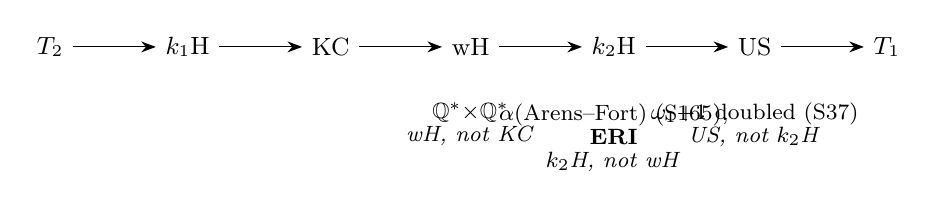
\begin{tikzpicture}[>={Stealth[scale=1.1]},
                    node distance=1.05cm,
                    every node/.style={font=\small}]
\node (T2)  {$T_2$};
\node[right=of T2]  (k1H) {$k_1\mathrm{H}$};
\node[right=of k1H] (KC)  {$\mathrm{KC}$};
\node[right=of KC]  (wH)  {$\mathrm{wH}$};
\node[right=of wH]  (k2H) {$k_2\mathrm{H}$};
\node[right=of k2H] (US)  {$\mathrm{US}$};
\node[right=of US]  (T1)  {$T_1$};
\draw[->] (T2)  -- (k1H);
\draw[->] (k1H) -- (KC);
\draw[->] (KC)  -- (wH);
\draw[->] (wH)  -- (k2H);
\draw[->] (k2H) -- (US);
\draw[->] (US)  -- (T1);
\node[below=10pt of wH,  align=center, font=\footnotesize]
  {$\mathbb{Q}^{\ast}{\times}\mathbb{Q}^{\ast}$\\[-1pt]
   \emph{wH, not KC}};
\node[below=10pt of k2H, align=center, font=\footnotesize]
  {$\alpha(\text{Arens--Fort})$ (S165),\\[-1pt]
   \textbf{ERI}\\[-1pt]
   \emph{$k_2$H, not wH}};
\node[below=10pt of US,  align=center, font=\footnotesize]
  {$\omega_1{+}1$ doubled (S37)\\[-1pt]
   \emph{US, not $k_2$H}};
\end{tikzpicture}
\end{center}

ERI occupies the $k_2$H-not-wH level alongside the one-point
compactification $\alpha(\text{Arens--Fort})$ (for the general theory
of compactifications, see Porter--Woods~\cite{bib:porterwoods}), but
the two are distinguished at every other axis:
$\alpha(\text{Arens--Fort})$ is totally disconnected and its non-$T_2$
point has countable pseudo-character, whereas ERI is
path-connected, sober, perfect, and has $\chi(\ast, X) \geq \aleph_1$.
The product $\mathbb{Q}^{\ast} \times \mathbb{Q}^{\ast}$ is weakly
Hausdorff and totally disconnected; the ordinal $\omega_1 + 1$ with
doubled endpoint is totally disconnected and fails $k_2$-Hausdorff.
None of the three is path-connected---this is the separation that
ERI supplies.

We now contrast ERI with the non-compact reference spaces.
The cocountable topology is US and KC but not compact; its only
convergent sequences are eventually constant.
ERI is compact, with a non-trivial convergence criterion
(Proposition~\ref{prop:seqconv}).
Van~Douwen's space is compact-US-KC, but its construction via MAD
families is highly non-constructive, and by K\"{u}nzi--van der
Zypen~\cite{bib:kunzi} every Fr\'{e}chet US-space is KC; ERI is
compact-US-not-KC and constructively explicit.
The line with two origins is first-countable and fails US (the sequence
$1/n$ converges to both origins); ERI is US and fails first-countability
precisely at $\ast$, and Fact~\ref{fact:firstUS} shows that
this trade-off is structurally necessary.
The standard quotient $(X_0, \tau_q)$ is Hausdorff; condition~(b)---the
density requirement on preimages of neighborhoods of $\ast$---is the
unique mechanism that destroys $T_2$ and KC while preserving $T_1$
and US.
The author is unaware of whether Van~Douwen's space is sober; see
Open Problem~\ref{op:vandouwen}.

\subsection{The $k_2$-Hausdorff property}\label{subsec:k2Hproof}

The $k_2$-Hausdorff property originates in the homotopical theory of
``convenient categories'' of topological spaces introduced by
Steenrod~\cite{bib:steenrod}, where closure of the diagonal in a
compactly generated setting is precisely the $k_2$H condition.
Within the refined Clontz hierarchy~\cite{bib:clontz,bib:clontzwilliams},
$k_2$H sits strictly between wH and US
(Remark~\ref{rmk:kspace} on the k-space of ERI).

\begin{definition}[$k_2$-Hausdorff]\label{def:k2H}
A space $X$ is \emph{$k_2$-Hausdorff} ($k_2$H) if for every compact
Hausdorff space $K$ and every continuous $f\colon K \to X$, the
\emph{kernel} $\ker(f) := \{(a,b) \in K^2 : f(a) = f(b)\}$ is closed
in $K \times K$.
Equivalently, for every pair
$k_0, k_1 \in K$ with $f(k_0) \neq f(k_1)$, there exist disjoint open
$U_0 \ni k_0$, $U_1 \ni k_1$ in $K$ with
$f[U_0] \cap f[U_1] = \varnothing$.
\end{definition}

This notion was introduced by
Clontz and Williams~\cite{bib:clontzwilliams}; we use the kernel
formulation (equivalent by~\cite[Prop.~2.3]{bib:clontzwilliams})
throughout.
The implications
$\mathrm{wH} \Rightarrow k_2\mathrm{H} \Rightarrow \mathrm{US}$
hold in general~\cite{bib:clontz}.

We prove the $k_2$H property in a general setting covering ERI and
every FMQ space over a first-countable base.
The notation below anticipates Section~\ref{sec:fmq}.

\begin{definition}[Filter-Modified Quotient, preview]\label{def:fmq-preview}
Let $(Y, \tau)$ be a topological space, $A \subseteq Y$ nonempty,
$q\colon Y \to Y/A$ the projection collapsing $A$ to
$\ast := q(A)$, and $\mathcal{F} \subseteq \mathcal{P}(Y)$ a
collection satisfying mild closure properties
(see Definition~\ref{def:admissible}).
The \emph{$\mathcal{F}$-modified quotient} is
$\mathrm{FMQ}(Y, A, \mathcal{F}) := (Y/A,\, \tau_{\mathcal{F}})$,
where $U \in \tau_{\mathcal{F}}$ iff $q^{-1}(U)$ is open in~$Y$
and ($\ast \in U \Rightarrow q^{-1}(U) \in \mathcal{F}$).
The \emph{density modifier} is
$\mathcal{D}_Y := \{D \subseteq Y : \overline{D} = Y\}$.
The original ERI is
$\mathrm{FMQ}(\overline{\mathbb{R}},\,\{-\infty,0,+\infty\},\,
\mathcal{D}_{\overline{\mathbb{R}}})$.
\end{definition}

Throughout this section, $Y$ is a compact Hausdorff space without
isolated points, $A \subseteq Y$ is finite, and
$X = \mathrm{FMQ}(Y, A, \mathcal{F})$ with $\mathcal{F} \subseteq
\mathcal{D}_Y$ and $X$ is $T_1$.

\begin{lemma}[Closed fibers principle]\label{lem:closedfibers}
Let $f\colon K \to X$ be continuous with $K$ compact Hausdorff. Set
$N := f^{-1}(\ast)$ and let $g\colon K \setminus N \to Y \setminus A$ be the
continuous ``coordinate map'' $g := (q|_{Y \setminus A})^{-1} \circ f$.
Then for every closed nowhere-dense $F \subset Y \setminus A$, the set
$g^{-1}(F)$ is closed in~$K$ \textup{(}not merely in $K \setminus N$\textup{)}.
\end{lemma}

\begin{proof}
Since $F$ is closed and nowhere dense, $Y \setminus F$ is open and dense.
Since $F \subset Y \setminus A$, we have $A \subseteq Y \setminus F$.
For $\mathcal{F} = \mathcal{D}_Y$: $Y \setminus F$ is dense, hence
$Y \setminus F \in \mathcal{D}_Y$.
More generally, closed nowhere-dense sets are meager, so when
$\mathcal{F}_{\mathrm{com}} \subseteq \mathcal{F}$,
$Y \setminus F$ is comeager, hence in $\mathcal{F}$.

Set $W_F := q(Y \setminus F)$. Then $\ast \in W_F$ and
$W_F \in \tau_{\mathcal{F}}$, so $f^{-1}(W_F)$ is open in~$K$.
Its complement is
$K \setminus f^{-1}(W_F) = \{k \in K \setminus N : g(k) \in F\}
= g^{-1}(F)$, which is therefore closed.
\end{proof}

\begin{proposition}[Accumulation structure]\label{prop:accum}
Suppose every point of $Y \setminus A$ has a countable neighborhood base
in~$Y$ \textup{(}automatic if $Y$ is metrizable\textup{)}.
Let $f$, $K$, $N$, $g$ be as in Lemma~\textup{\ref{lem:closedfibers}}.
If $(k_\alpha)$ is a net in $K \setminus N$ with $k_\alpha \to a \in N$,
then every cluster point of $(g(k_\alpha))$ in~$Y$ belongs to~$A$.
\end{proposition}

\begin{proof}
Suppose a subnet $g(k_{\alpha_j}) \to z$ with $z \in Y \setminus A$;
we derive a contradiction.

\emph{Step~1.}
Since $\{z\}$ is closed and nowhere dense ($z$ is not isolated),
Lemma~\ref{lem:closedfibers} gives $g^{-1}(\{z\})$ closed in~$K$.
Because $a \in N$ and $g^{-1}(\{z\}) \subseteq K \setminus N$, we have
$a \notin g^{-1}(\{z\})$, so $k_{\alpha_j} \notin g^{-1}(\{z\})$
eventually, i.e., $g(k_{\alpha_j}) \neq z$ eventually.

\emph{Step~2 (sequence extraction).}
Since $z \in Y \setminus A$ has a countable neighborhood base
$V_1 \supset V_2 \supset \cdots$, the set
$R_n := \{j : g(k_{\alpha_j}) \in V_n \setminus \{z\}\}$ is cofinal
in the directed set.
Pick $j_1 \in R_1$. For $n \ge 2$, pick $j_n \in R_n$ with
$j_n \ge j_{n-1}$ and
$g(k_{\alpha_{j_n}}) \notin
\{g(k_{\alpha_{j_1}}), \ldots, g(k_{\alpha_{j_{n-1}}})\}$
(possible since each $g^{-1}(\{v\})$ is closed in~$K$ by
Lemma~\ref{lem:closedfibers} with $a \notin g^{-1}(\{v\})$;
the finite intersection of cofinal sets with $R_n$ is cofinal).

\emph{Step~3.}
Define $C := \{g(k_{\alpha_{j_n}}) : n \ge 1\} \cup \{z\}$.
The values are distinct and $g(k_{\alpha_{j_n}}) \to z$, so $z$ is the
only accumulation point of~$C$ and $z \in C$, hence $C$ is closed.
$C \subset Y \setminus A$ is countable, hence meager (each singleton is
nowhere dense since $Y$ has no isolated points), hence nowhere dense
(closed and meager in a Baire
space~\cite[Theorem~3.9.3]{bib:engelking}).

\emph{Step~4.}
By Lemma~\ref{lem:closedfibers}, $g^{-1}(C)$ is closed in~$K$.
Since $k_{\alpha_{j_n}} \in g^{-1}(C)$ for all~$n$ and
$k_{\alpha_{j_n}} \to a$, we get
$a \in \overline{g^{-1}(C)} = g^{-1}(C) \subseteq K \setminus N$.
But $a \in N$---contradiction.
\end{proof}

\begin{theorem}[$k_2$-Hausdorff for FMQ spaces]\label{thm:k2H}
Let $Y$ be a compact Hausdorff space without isolated points,
$A \subseteq Y$ finite, and $\mathcal{F}$ an admissible modifier with
$\mathcal{F} \subseteq \mathcal{D}_Y$.
Suppose every point of $Y \setminus A$ has a countable neighborhood base
in~$Y$ \textup{(}automatic if $Y$ is metrizable\textup{)}, and suppose
$X = \mathrm{FMQ}(Y, A, \mathcal{F})$ is $T_1$. Then $X$ is
$k_2$-Hausdorff.

In particular, ERI $= \mathrm{FMQ}(\overline{\mathbb{R}},
\{-\infty,0,+\infty\}, \mathcal{D}_{\overline{\mathbb{R}}})$ is
$k_2$-Hausdorff.
\end{theorem}

\begin{proof}
We show that $\ker(f) := \{(a,b) \in K^2 : f(a) = f(b)\}$ is closed
in $K^2$ for every compact Hausdorff~$K$ and continuous
$f\colon K \to X$.
Let $(k_\alpha, \ell_\alpha)$ be a net in $\ker(f)$ converging to $(a,b)$.
By continuity, $f(k_\alpha) \to f(a)$ and $f(\ell_\alpha) \to f(b)$;
since $f(k_\alpha) = f(\ell_\alpha)$, the common net converges to both
$f(a)$ and $f(b)$.

Set $X_0 := X \setminus \{\ast\} \cong Y \setminus A$ (Hausdorff).

\emph{Case~1: $f(a), f(b) \in X_0$.}
The net $f(k_\alpha)$ is eventually in $X_0$ (since $\{\ast\}$ is closed
and $f(a) \neq \ast$). In the Hausdorff space $X_0$, a net has at most
one limit, so $f(a) = f(b)$.

\emph{Case~2: $f(a) = f(b) = \ast$.} Immediate.

\emph{Case~3: $f(a) = \ast$, $f(b) = \hat{r}$ with
$r \in Y \setminus A$} (or vice versa).
We derive a contradiction.
Since $\hat{r} \neq \ast$ and $\{\ast\}$ is closed, eventually
$f(\ell_\alpha) \in X_0$, so $\ell_\alpha \in K \setminus N$ eventually.
Since $f(k_\alpha) = f(\ell_\alpha) \neq \ast$ eventually,
both $k_\alpha$ and $\ell_\alpha$ eventually lie in $K \setminus N$,
where $g$ is defined.
The injectivity of $q|_{Y \setminus A}$ gives
$g(k_\alpha) = g(\ell_\alpha)$.
Since $\ell_\alpha \to b$ and $g(b) = r$: $g(\ell_\alpha) \to r$, so
$g(k_\alpha) \to r$.
But $k_\alpha \to a \in N$, so by Proposition~\ref{prop:accum} every
cluster point of $(g(k_\alpha))$ lies in~$A$. In particular,
$g(k_\alpha)$ cannot converge to $r \in Y \setminus A$---contradiction.
\end{proof}

\begin{remark}\label{rem:k2Hgeneral}
The first-countability hypothesis on $Y \setminus A$ is used in Step~2
of Proposition~\ref{prop:accum} to extract a convergent \emph{sequence}
of values. It is satisfied by every metrizable~$Y$, hence by all
standard examples ($\overline{\mathbb{R}}$, $[0,1]$, $S^1$, the Cantor
set, $[0,1]^\omega$, etc.).
A complete proof for non-first-countable~$Y$ (such as
$\beta\mathbb{N} \setminus \mathbb{N}$) remains an open question.
\end{remark}

\begin{remark}\label{rmk:k2H-method}
The key to Theorem~\ref{thm:k2H} is the interplay between two facts:
\begin{enumerate}[nosep]
\item Proposition~\ref{prop:accum}: the density condition forces
  $g(k_\alpha) \to L$ with $L \in Y \setminus A$ to be
  incompatible with $k_\alpha \to a \in f^{-1}(\ast)$.
\item The $T_1$ property: $\{\ast\}$ is closed, so convergence to
  $\hat{r} \neq \ast$ eventually places the net in $X \setminus
  \{\ast\}$, enabling the coordinate map argument.
\end{enumerate}
This places ERI at the same level as the one-point
compactification of the Arens--Fort space ($k_2$H but not~wH;
see~\cite{bib:clontz}).
\end{remark}

\subsection{Refined hierarchy placement}\label{sec:position}

We now locate ERI in the refined hierarchy of
Clontz~\cite{bib:clontz}:
$T_2 \Rightarrow \mathrm{k_1H} \Rightarrow \mathrm{KC}
\Rightarrow \mathrm{wH} \Rightarrow \mathrm{k_2H}
\Rightarrow \mathrm{US} \Rightarrow T_1$,
and in the chain of Bella and
Costantini~\cite{bib:bella}: $\mathrm{KC} \Rightarrow \mathrm{SC}
\Rightarrow \mathrm{US}$, where a space is \emph{SC} (sequentially
closed) if every convergent sequence together with its limit is a
closed set.

\begin{proposition}\label{prop:notwH}
ERI is not weakly Hausdorff.
\end{proposition}
\begin{proof}
A space is \emph{weakly Hausdorff} (wH) if every continuous image of a
compact Hausdorff space is closed~\cite{bib:clontz}.
The map $f\colon [0,1] \to X$ defined by $f(t) = q(t+1)$ is continuous
(composition of $q$ with the continuous map $t \mapsto t+1\colon [0,1] \to [1,2]$;
note that $[1,2] \subset \mathbb{R}\setminus\{0\}$, so $f$ does not
pass through~$\ast$) and $[0,1]$ is compact
Hausdorff.
The image $f([0,1]) = q([1,2])$ is not closed:
$\ast \in X \setminus q([1,2])$ (since $[1,2] \subset
\mathbb{R}\setminus\{0\}$), but
$q^{-1}(X \setminus q([1,2])) = \overline{\mathbb{R}} \setminus [1,2]$
is not dense (the complement $[1,2]$ has interior $(1,2)$), so
condition~(b) fails.
\end{proof}

\begin{proposition}\label{prop:SC}
ERI is SC \textup{(sequentially closed)}.
\end{proposition}
\begin{proof}
Let $(y_n)$ be a convergent sequence in~$X$ with limit~$L$, and set
$S := \{y_n : n \ge 1\} \cup \{L\}$.
We show $X \setminus S \in \tau_{\mathrm{ERI}}$.

\emph{Case $L = \hat{c}$, $c \in \mathbb{R}\setminus\{0\}$.}\;
Write $y_n = q(x_n)$ with $x_n \to c$.
Then $S \subset X \setminus \{\ast\}$
and $\ast \in X \setminus S$.
The set $C := \{c\} \cup \{x_n : n \ge 1\}$ is countable, closed in
$\overline{\mathbb{R}}$ (limit point $c$ included), and nowhere dense.
Hence $q^{-1}(X \setminus S) = \overline{\mathbb{R}} \setminus C$
is open and dense.

\emph{Case $L = \ast$.}\;
By Proposition~\ref{prop:seqconv}, $(x_n)$ has no accumulation point
in $\mathbb{R}\setminus\{0\}$; every accumulation point in
$\overline{\mathbb{R}}$ belongs to $\{-\infty, 0, +\infty\}$.
Since $\ast \in S$, we have $\ast \notin X \setminus S$, so
condition~(b) does not apply to $X \setminus S$.
The set $\{-\infty, 0, +\infty\} \cup \{x_n : n \ge 1\}$ is closed
in $\overline{\mathbb{R}}$ (all limit points of $\{x_n\}$ lie
in $\{-\infty, 0, +\infty\}$ and are included), so
$q^{-1}(X \setminus S)$ is open.
\end{proof}

\begin{proposition}\label{prop:seqcpt}
ERI is sequentially compact.
\end{proposition}
\begin{proof}
Let $(y_n)$ be a sequence in~$X$.
If $y_n = \ast$ for infinitely many~$n$, the constant subsequence
converges.
Otherwise, $y_n = q(x_n)$ with $x_n \in \mathbb{R}\setminus\{0\}$
for all large~$n$.
Since $\overline{\mathbb{R}}$ is compact and metrizable, it is
sequentially compact, so $(x_n)$ has a subsequence
$x_{n_k} \to L \in \overline{\mathbb{R}}$.
If $L \in \mathbb{R}\setminus\{0\}$, then $q(x_{n_k}) \to \hat{L}$
(the subspace topology on $X \setminus \{\ast\}$ agrees with the
Euclidean topology).
If $L \in \{-\infty, 0, +\infty\}$, then every accumulation point
of $(x_{n_k})$ in $\overline{\mathbb{R}}$ is~$L$, which lies in
$\{-\infty, 0, +\infty\}$; by
Proposition~\ref{prop:seqconv}, $q(x_{n_k}) \to \ast$.
\end{proof}

\begin{remark}[Sequential compactness preservation]\label{rmk:SCpreserv}
More generally, if $Y$ is sequentially compact, then
$X = \mathrm{FMQ}(Y, A, \mathcal{F})$ is sequentially compact for
any admissible modifier~$\mathcal{F}$: subsequential limits in~$Y$
project to limits in~$X$ via~$q$.
\end{remark}

\begin{theorem}[Sobriety]\label{thm:sober}
$(X, \tau_{\mathrm{ERI}})$ is sober.
\end{theorem}

\begin{proof}
A space is \emph{sober} if every irreducible closed subset has a unique
generic point.  A closed set~$F$ is \emph{irreducible} if whenever
$F = F_1 \cup F_2$ with $F_1, F_2$ closed, then $F_1 = F$ or $F_2 = F$.
A point~$x$ is \emph{generic} for~$F$ if $\overline{\{x\}} = F$.

Since $X$ is~$T_1$ (Proposition~\ref{prop:T1}), every singleton is
closed, so $\overline{\{x\}} = \{x\}$ for all $x \in X$.  Hence a closed
set can have a generic point only if it is a singleton, and each
singleton~$\{x\}$ has the unique generic point~$x$.  Sobriety therefore
reduces to the following claim.

\medskip
\noindent\textbf{Claim.}\; \emph{Every closed subset $F \subseteq X$
with $|F| \geq 2$ is reducible} (i.e., expressible as a union of two
proper closed subsets).
\medskip

\noindent\emph{Case 1: $\ast \notin F$.}\;
Then $F \subseteq X \setminus \{\ast\}$.  The subspace
$X \setminus \{\ast\}$ carries the Euclidean topology of
$\mathbb{R}\setminus\{0\}$ (since $q$ restricts to a homeomorphism
$\mathbb{R}\setminus\{0\} \xrightarrow{\;\sim\;} X\setminus\{\ast\}$),
hence is Hausdorff.  Every Hausdorff space is sober: if $|F| \geq 2$,
pick distinct $a, b \in F$ and separate them by disjoint open sets
$U_a, U_b$ in the subspace; then $F = (F \setminus U_a) \cup (F \setminus U_b)$
is a decomposition into two proper closed subsets of~$F$.
Since irreducibility is intrinsic to the subspace topology on~$F$,
the set~$F$ is reducible.

\smallskip
\noindent\emph{Case 2: $\ast \in F$ and $|F| \geq 2$.}\;
Pick $\hat{c} \in F \setminus \{\ast\}$ with
$c \in \mathbb{R}\setminus\{0\}$.  Choose $\varepsilon > 0$ small
enough that $[c - \varepsilon,\, c + \varepsilon] \subseteq
\mathbb{R}\setminus\{0\}$ (possible since $c \neq 0$).  Define
\[
  K \;:=\; q\bigl([c-\varepsilon,\, c+\varepsilon]\bigr),
  \qquad
  L \;:=\; X \setminus q\bigl((c-\varepsilon,\, c+\varepsilon)\bigr).
\]
We verify that $K$ and $L$ are closed in~$X$.

\emph{$K$ is closed.}\;
Its complement satisfies
$q^{-1}(X \setminus K) = \overline{\mathbb{R}} \setminus
[c-\varepsilon, c+\varepsilon]$, which is open in~$\overline{\mathbb{R}}$.
Moreover, $\{-\infty, 0, +\infty\} \subseteq
\overline{\mathbb{R}} \setminus [c-\varepsilon,c+\varepsilon]$
(since $[c-\varepsilon,c+\varepsilon] \subseteq
\mathbb{R}\setminus\{0\}$), and
$\overline{\mathbb{R}} \setminus [c-\varepsilon,c+\varepsilon]$
is dense in~$\overline{\mathbb{R}}$ because it contains
$(-\infty, c-\varepsilon) \cup (c+\varepsilon, +\infty)$.
Since $\ast \in X \setminus K$, condition~(b) requires this density,
which holds.  So $X \setminus K \in \tau_{\mathrm{ERI}}$.

\emph{$L$ is closed.}\;
Its complement satisfies
$q^{-1}(X \setminus L) = (c-\varepsilon, c+\varepsilon)$, which is open
in~$\overline{\mathbb{R}}$.
Since $\ast \notin X \setminus L$ (as
$\{-\infty, 0, +\infty\} \cap (c-\varepsilon,c+\varepsilon) = \varnothing$),
condition~(b) is vacuous.  So $X \setminus L \in \tau_{\mathrm{ERI}}$.

Now set $F_1 := F \cap K$ and $F_2 := F \cap L$.  Both are closed
(intersections of closed sets).  We check the three required properties.
\begin{itemize}[nosep]
\item \emph{$F_1 \subsetneq F$:}\;
  Since $q^{-1}(K) = [c-\varepsilon,c+\varepsilon]$ does not meet
  $\{-\infty,0,+\infty\}$, we have $\ast \notin K$, hence
  $\ast \notin F_1$.  But $\ast \in F$, so $F_1 \subsetneq F$.
  Also $\hat{c} \in K \cap F$ gives $F_1 \neq \varnothing$.
\item \emph{$F_2 \subsetneq F$:}\;
  Since $c \in (c-\varepsilon,c+\varepsilon)$, we have
  $\hat{c} \in q\bigl((c-\varepsilon,c+\varepsilon)\bigr)$, hence
  $\hat{c} \notin L$ and $\hat{c} \notin F_2$.  But $\hat{c} \in F$,
  so $F_2 \subsetneq F$.
  Also $\ast \notin q\bigl((c-\varepsilon,c+\varepsilon)\bigr)$ gives
  $\ast \in L$, so $\ast \in F_2 \neq \varnothing$.
\item \emph{$F_1 \cup F_2 = F$:}\;
  It suffices to show $K \cup L = X$.  Let $\hat{x} \in X$.  If
  $\hat{x} \in K$ we are done.  If $\hat{x} \notin K$, then
  $x \notin [c-\varepsilon, c+\varepsilon]$, so in particular
  $x \notin (c-\varepsilon, c+\varepsilon)$, hence
  $\hat{x} \notin q\bigl((c-\varepsilon,c+\varepsilon)\bigr)$, giving
  $\hat{x} \in L$.
\end{itemize}
Thus $F = F_1 \cup F_2$ with both $F_i$ proper closed subsets
of~$F$; hence $F$ is reducible.

\medskip
In both cases every closed set with $|F| \geq 2$ is reducible.
The only irreducible closed sets are the singletons~$\{x\}$, each with
unique generic point~$x$.  Hence $(X, \tau_{\mathrm{ERI}})$ is sober.
\end{proof}

\begin{remark}[Sobriety vs.\ connectedness]\label{rmk:sober-subtlety}
It may seem surprising that a $T_1$, connected, non-Hausdorff space
can be sober.
The classical counterexample to sobriety in $T_1$ spaces is the
\emph{cocountable topology} on an uncountable set, where the whole
space is irreducible with no generic point.
The key distinction is between \emph{connectedness} (no partition
into two disjoint non-empty closed sets) and \emph{irreducibility}
(no expression as a union of two proper closed subsets, which may
overlap).
In ERI the closed sets $F_1 = F \cap K$ and $F_2 = F \cap L$
constructed in Case~2 above overlap---they share points of~$F$
other than $\ast$ and $\hat{c}$---so the decomposition
$F = F_1 \cup F_2$ does not contradict connectedness.
\end{remark}

\begin{remark}[Position summary]\label{rmk:position}
Combining the results of this paper, ERI occupies the position
marked with~$\bullet$ in the following Hasse diagram of the
Clontz hierarchy~\cite{bib:clontz}~\eqref{eq:clontz}
(an arrow $P \to Q$ means $P \Rightarrow Q$;
labels indicate ERI's status):

\begin{center}
\begin{tikzpicture}[
  node distance=0.9cm,
  level/.style={font=\normalsize},
  no/.style={font=\scriptsize, text=red!70!black},
  yes/.style={font=\scriptsize, text=green!50!black},
  >={Stealth[length=4pt]}
]
\node[level] (T2) {$T_2$};
\node[level, below=of T2] (k1H) {$\mathrm{k_1H}$};
\node[level, below=of k1H] (KC) {$\mathrm{KC}$};
\node[level, below=of KC] (wH) {$\mathrm{wH}$};
\node[level, below=of wH, draw, thick, inner sep=4pt, rounded corners=2pt,
      fill=blue!5] (k2H) {$\mathrm{k_2H}$};
\node[level, below=of k2H] (US) {$\mathrm{US}$};
\node[level, below=of US] (T1) {$T_1$};

% ERI status labels (right of each node)
\node[no, right=4pt of T2] {$\times$};
\node[no, right=4pt of k1H] {$\times$};
\node[no, right=4pt of KC] {$\times$};
\node[no, right=4pt of wH] {$\times$};
\node[yes, right=10pt of k2H] {$\checkmark$};
\node[yes, right=4pt of US] {$\checkmark$};
\node[yes, right=4pt of T1] {$\checkmark$};

\draw[->] (T2) -- (k1H);
\draw[->] (k1H) -- (KC);
\draw[->] (KC) -- (wH);
\draw[->] (wH) -- (k2H);
\draw[->] (k2H) -- (US);
\draw[->] (US) -- (T1);

% Side info panel — anchored at T2 level
\node[right=3.2cm of T2, anchor=north west, text width=4.2cm,
      font=\small] (side) {%
  $\mathrm{KC} \Rightarrow \mathrm{SC}
   \Rightarrow \mathrm{US}$\\[2pt]
  ERI: SC\,=\,Yes, KC\,=\,No\\[6pt]
  Sober, compact,\\
  path-connected, loc.\ connected\\[4pt]
  $t(\ast) = \aleph_0$,\;
  $\chi(\ast) \geq \aleph_1$};

% "ERI is here" label — left side
\node[left=1.5cm of k2H, font=\small, text=blue!70!black]
  (erihere) {\textbf{ERI is here}};
\draw[->, blue!70!black, shorten >=2pt]
  (erihere.east) -- (k2H.west);
\end{tikzpicture}
\end{center}

\noindent
Theorem~\ref{thm:k2H} places ERI at the same hierarchy level~\cite{bib:clontz} as the
one-point compactification of the Arens--Fort space:
both are $k_2$H but not wH.
ERI is the only known path-connected
compact sober example at this level.
\end{remark}

\subsection{Regularity failures}

\begin{proposition}[Functional triviality for ERI]\label{prop:ERI-cfunctions}
Every continuous function $f\colon X \to \mathbb{R}$ is constant.
\end{proposition}
\begin{proof}
Let $g := f \circ q\colon \overline{\mathbb{R}} \to \mathbb{R}$;
then $g$ is continuous and
$g(-\infty) = g(0) = g(+\infty) =: c$.
Suppose $g(t) \neq c$ for some $t \in \mathbb{R}\setminus\{0\}$.
Pick $\varepsilon < |g(t) - c|/2$.
The set $U := f^{-1}((c - \varepsilon, c + \varepsilon))$ is open
in~$X$ with $\ast \in U$, so $q^{-1}(U)$ must be dense.
But
$q^{-1}(U) = g^{-1}((c - \varepsilon, c + \varepsilon))$
misses the nonempty open set
$g^{-1}((g(t) - \varepsilon, g(t) + \varepsilon))$---contradicting density.
\end{proof}

\begin{corollary}[Pseudocompactness of ERI]\label{cor:ERI-pseudocompact}
ERI is pseudocompact: every continuous $f\colon X \to \mathbb{R}$
is bounded \textup{(}indeed constant\textup{)}.
\end{corollary}

\begin{corollary}\label{cor:ERI-notCR}
ERI is not completely regular.
\end{corollary}
\begin{proof}
A completely regular space with more than one point admits a non-constant
continuous function to $\mathbb{R}$; by
Proposition~\ref{prop:ERI-cfunctions}, no such function exists.
\end{proof}

\begin{corollary}\label{cor:ERI-notregular}
ERI is not regular \textup{(}$T_3$\textup{)}.
\end{corollary}
\begin{proof}
If ERI were regular, then $T_1 +$ regular $= T_3 \Rightarrow T_2$,
and compact $T_2 \Rightarrow$ normal
(\cite{bib:engelking},~Theorem~3.1.9, under the convention
compact $=$ quasi-compact $+$ Hausdorff).
Then normal $+$ $T_1$ $\Rightarrow$ completely regular (Urysohn lemma),
contradicting Corollary~\ref{cor:ERI-notCR}.
Alternatively, the KIP
(Proposition~\ref{prop:kip}) shows directly that $\ast$ and any
closed set $\{\hat{c}\}$ ($c \neq 0$) cannot be separated by disjoint
open sets.
\end{proof}

\begin{corollary}\label{cor:ERI-notnormal}
ERI is not normal.
\end{corollary}
\begin{proof}
By the Urysohn lemma, every normal $T_1$ space is completely regular.
ERI is $T_1$ (Proposition~\ref{prop:T1}) but not completely regular.
\end{proof}

\begin{proposition}[Hausdorff-valued maps are constant]\label{prop:hausdorff-constant}
Every continuous map from $X$ to a Hausdorff space with at least two
points is constant.
In particular, $\check{H}^n(X;\mathbb{Z}) = 0$ for all $n \geq 1$
\textup{(}\v{C}ech cohomology\textup{)}.
\end{proposition}
\begin{proof}
Let $f\colon X \to T$ be continuous with $T$ Hausdorff and $|T| \geq 2$.
Set $c := f(\ast)$.
Suppose $f(\hat{x}) \neq c$ for some $\hat{x} \in X$.
Since $T$ is Hausdorff, separate $f(\hat{x})$ and $c$ by disjoint
open sets $V_{x} \ni f(\hat{x})$ and $V_c \ni c$.
Then $U := f^{-1}(V_c)$ is open in~$X$ with $\ast \in U$, and
$W := f^{-1}(V_x)$ is nonempty and open.
The KIP (Proposition~\ref{prop:kip}) gives $U \cap W \neq \varnothing$,
but $V_c \cap V_x = \varnothing$---contradiction.
For cohomology: for each $n \geq 1$, the Eilenberg--MacLane space
$K(\mathbb{Z}, n)$ is Hausdorff (it is a CW-complex), so every
continuous map $X \to K(\mathbb{Z}, n)$ is constant.
By the representability of \v{C}ech cohomology on compact spaces
(\cite{bib:engelking},~\S3.7; see also~\cite{bib:munkres},~\S73),
$\check{H}^n(X;\mathbb{Z}) \cong [X, K(\mathbb{Z}, n)] = 0$
for all $n \geq 1$.
\end{proof}

\subsection{Summary: ERI in the hierarchy}

Combining the results of
Sections~\ref{sec:construction}--\ref{sec:position}, the topological
profile of ERI can be stated compactly.
ERI is $T_1$ (Proposition~\ref{prop:T1}), US (Theorem~\ref{thm:US}),
sequentially closed (Proposition~\ref{prop:SC}), $k_2$-Hausdorff
(Theorem~\ref{thm:k2H}), and sober (Theorem~\ref{thm:sober}); it fails
weakly Hausdorff (Proposition~\ref{prop:notwH}), KC
(Theorem~\ref{thm:notKC}), and Hausdorff
(Theorem~\ref{thm:nothausdorff}).
It is compact, sequentially compact
(Proposition~\ref{prop:seqcpt}), pseudocompact
(Corollary~\ref{cor:ERI-pseudocompact}), a $k$-space
(Remark~\ref{rmk:kspace}), path-connected
(Proposition~\ref{prop:pathconn}), locally connected
(Proposition~\ref{prop:localconn}), separable
(Remark~\ref{rmk:separable}), ccc, and Baire
(Proposition~\ref{prop:baire}).
It fails first-countability at $\ast$
(Proposition~\ref{prop:notfirst}) and is neither sequential nor
Fr\'{e}chet--Urysohn
(Proposition~\ref{prop:notsequential}).
The regularity axioms all fail: ERI is not regular, completely regular,
semiregular, normal, or metrizable
(Corollaries~\ref{cor:ERI-notregular}, \ref{cor:ERI-notCR},
\ref{cor:ERI-notnormal}; Remarks~\ref{rmk:semiregular},
\ref{rmk:submetrizable}), though it is paracompact.
The continuous function space $C(X, \mathbb{R})$ consists of constants
only (Proposition~\ref{prop:ERI-cfunctions}), every continuous map
from~$X$ to a Hausdorff space is constant, and
$\check{H}^n(X; \mathbb{Z}) = 0$ for all $n \geq 1$
(Proposition~\ref{prop:hausdorff-constant}).
The relevant cardinal invariants are
$t(\ast, X) = \aleph_0$, $\chi(\ast, X) \geq \aleph_1$,
$w(X) = \mathfrak{c}$, $c(X) = s(X) = \aleph_0$, and
$\mathrm{ind}(X) = 1$
(Propositions~\ref{prop:notfirst}, \ref{prop:tightness},
\ref{prop:cardinal}, \ref{prop:dim}; Remark~\ref{rmk:weight}).

ERI is \emph{perfect}: every point of
$X \setminus \{\ast\} \cong \mathbb{R} \setminus \{0\}$ is a limit
point, and $\ast$ belongs to the closure of every nonempty open set
(Corollary~\ref{cor:pclosure}).
Hence ERI provides a concrete, compact, path-connected witness of the
strict implication $\mathrm{KC} \Rightarrow \mathrm{US}$---that is, of
$\mathrm{US} \not\Rightarrow \mathrm{KC}$---arising from an elementary
quotient construction.

% =================================================================
\section{The Filter-Modified Quotient Framework}\label{sec:fmq}
% =================================================================

The preceding sections establish ERI as a concrete example with a
specific base space ($\overline{\mathbb{R}}$) and collapse set
($\{-\infty,0,+\infty\}$).
A natural question is whether the construction is ad hoc---tied to the
peculiarities of the real line---or reflects a deeper structural
phenomenon.
We now develop the \emph{Filter-Modified Quotient} (FMQ)
framework, which shows that the density condition is a calibrated
mechanism producing the same hierarchy level for \emph{any}
compact Hausdorff base without isolated points.
Specifically, this framework yields three results not
visible from ERI alone: a modifier spectrum revealing the density
condition as an optimal equilibrium
(Sections~\ref{sec:modifiers}--\ref{sec:optimality}), an abstract
characterization of the US zone (Section~\ref{sec:convergence}),
and an extended rigidity analysis showing that the hierarchy level
is invariant under infinite collapse sets, iteration, and products
(Section~\ref{sec:extended}).
Several ERI-specific results
(convergence criterion, SC, sobriety, functional triviality) are
special cases of their FMQ counterparts below; we state the general
versions and indicate where the ERI proofs carry over
\emph{verbatim}.

\subsection{Admissible modifiers and the FMQ construction}

\begin{definition}[Admissible modifier]\label{def:admissible}
Let $(X, \tau)$ be a topological space.  A collection
$\mathcal{F} \subseteq \mathcal{P}(X)$ is a
\emph{$\tau$-admissible modifier} if:
\begin{enumerate}[label=\textup{(F\arabic*)},nosep]
\item\label{F1} $X \in \mathcal{F}$.
\item\label{F2} $\mathcal{F}$ is upward closed: $F \in \mathcal{F}$
      and $F \subseteq G$ implies $G \in \mathcal{F}$.
\item\label{F3} If $U_1, U_2 \in \mathcal{F} \cap \tau$, then
      $U_1 \cap U_2 \in \mathcal{F}$.
\end{enumerate}
\end{definition}

\begin{definition}[Filter-Modified Quotient]\label{def:fmq}
Let $(X, \tau)$ be a topological space, $A \subseteq X$ nonempty,
$q\colon X \to X/A$ the projection collapsing $A$ to
$\ast := q(A)$, and $\mathcal{F}$ a $\tau$-admissible modifier.
The \emph{$\mathcal{F}$-modified quotient topology} is
\[
\tau_{\mathcal{F}} \;:=\;
\bigl\{\, U \subseteq X/A :
  q^{-1}(U) \in \tau \;\;\text{and}\;\;
  \bigl(\ast \in U \Longrightarrow q^{-1}(U) \in \mathcal{F}\bigr)
\,\bigr\}.
\]
We write $\mathrm{FMQ}(X, A, \mathcal{F}) := (X/A,\,
\tau_{\mathcal{F}})$.
\end{definition}

\begin{proposition}\label{prop:fmq-top}
$\tau_{\mathcal{F}}$ is a topology on $X/A$, with
$\tau_{\mathcal{F}} \subseteq \tau_q$ \textup{(}the standard quotient
topology\textup{)} and equality on subsets not containing~$\ast$.
Moreover, $q\colon (X, \tau) \to (X/A, \tau_{\mathcal{F}})$ is
continuous.
\end{proposition}

\begin{proof}
$\varnothing \in \tau_{\mathcal{F}}$ (vacuous) and
$X/A \in \tau_{\mathcal{F}}$ (since $X \in \mathcal{F}$
by~\ref{F1}).
For finite intersections: if $\ast \in U_1 \cap U_2$, then
$q^{-1}(U_i) \in \mathcal{F} \cap \tau$, and~\ref{F3} gives
$q^{-1}(U_1) \cap q^{-1}(U_2) \in \mathcal{F}$.
For arbitrary unions: if $\ast \in \bigcup_i U_i$, pick $j$ with
$\ast \in U_j$; then $q^{-1}(U_j) \in \mathcal{F}$ and
$q^{-1}(U_j) \subseteq \bigcup_i q^{-1}(U_i)$, so~\ref{F2} gives
$\bigcup_i q^{-1}(U_i) \in \mathcal{F}$.
The remaining assertions are immediate from the definition.
\end{proof}

\begin{proposition}\label{prop:dense-admissible}
The collection of dense subsets
$\mathcal{D}_X := \{D \subseteq X : \overline{D} = X\}$
is a $\tau$-admissible modifier on any topological space~$(X,\tau)$.
\textup{(}Note: $\mathcal{D}_X$ is not a filter in general---$\mathbb{Q}$
and $\mathbb{R} \setminus \mathbb{Q}$ are both dense with empty
intersection---but the weaker axiom~\textup{\ref{F3}} suffices.\textup{)}
\end{proposition}

\begin{proof}
\ref{F1}:~$X$ is dense.
\ref{F2}:~supersets of dense sets are dense.
\ref{F3}:~finite intersections of dense open sets are
dense~\cite[1.3.5]{bib:engelking}.
\end{proof}

\begin{remark}\label{rmk:eri-fmq}
The requirement that $A$ be closed is essential for $T_1$
(see row~9 of Appendix~\ref{app:master}).
The original ERI is
$\mathrm{FMQ}(\overline{\mathbb{R}},\,\{-\infty,0,+\infty\},\,
\mathcal{D}_{\overline{\mathbb{R}}})$;
the generalized ERI of Theorem~\ref{thm:general} is
$\mathrm{FMQ}(Y, A, \mathcal{D}_Y)$.
\end{remark}

\subsection{Basic properties of FMQ spaces}

\begin{proposition}\label{prop:fmq-basic}
Let $Y$ be a topological space, $A \subseteq Y$ finite nonempty, and
$\mathcal{F}$ an admissible modifier.
\begin{enumerate}[label=\textup{(\roman*)},nosep]
\item If $Y$ is compact, then $\mathrm{FMQ}(Y, A, \mathcal{F})$ is compact.
\item $\mathrm{FMQ}(Y, A, \mathcal{F})$ is $T_1$ if and only if: $Y$ is $T_1$,
  $A$ is closed in~$Y$, and for every
  $y \in Y \setminus A$, $Y \setminus \{y\} \in \mathcal{F}$.
\end{enumerate}
\end{proposition}

\begin{proof}
(i) follows from compactness of $Y$ and continuity of $q$.
For~(ii): the singleton $\{\ast\}$ is closed iff
$X \setminus \{\ast\}$ is open; its preimage is $Y \setminus A$,
and $\ast \notin X \setminus \{\ast\}$, so the $\mathcal{F}$-condition
is vacuous.  Hence $\{\ast\}$ is closed iff $Y \setminus A$ is open,
i.e., iff $A$ is closed in~$Y$.
For $y \notin A$: $\{\hat{y}\}$ is closed iff $X \setminus \{\hat{y}\}$ is open; the preimage is $Y \setminus \{y\}$ which contains~$A$, so both conditions
(open $+$ $\mathcal{F}$-membership) must hold.
\end{proof}

\subsection{The generalized ERI construction}

The density modifier $\mathcal{D}_Y$ applied to any compact Hausdorff
base without isolated points yields a US-not-KC space:

\begin{lemma}\label{lem:infinite}
A Hausdorff space with no isolated points and at least one point is
infinite.
\end{lemma}

\begin{proof}
If $X$ is finite and Hausdorff, every singleton is open (finite $T_1$
spaces are discrete), so every point is isolated.
\end{proof}

\begin{theorem}[Generalized ERI construction]\label{thm:general}
Let $Y$ be a compact Hausdorff space with no isolated points, and let
$A = \{a_1, \ldots, a_k\} \subset Y$ ($k \geq 1$) be a finite non-empty
subset.
Then $X := \mathrm{FMQ}(Y, A, \mathcal{D}_Y)$ is:
\begin{enumerate}[label=\textup{(\alph*)},nosep]
\item compact;
\item $T_1$;
\item not Hausdorff;
\item connected;
\item US;
\item not KC.
\end{enumerate}
\end{theorem}
\begin{proof}
\emph{Parts (a)--(b).}\; Follow from
Proposition~\ref{prop:fmq-basic}.

\emph{Part (c).}\; The density modifier satisfies
\textup{(KIP$_{\mathcal{F}}$)} (Remark~\ref{rem:KIPdensity} below),
so every neighborhood of $\ast$ meets every nonempty open set.

\emph{(d) Connected.}\;
Suppose $X = U \cup V$ is a disconnection with $\ast \in U$.
Then $q^{-1}(U)$ is open and dense, and $q^{-1}(V)$ is open and nonempty.
A dense set meets every nonempty open set, so
$q^{-1}(U) \cap q^{-1}(V) \neq \varnothing$, contradicting
$U \cap V = \varnothing$.

\emph{(e) US.}\;
This follows from Lemma~\ref{lem:baire} (Baire exclusion) below.

\emph{(f) Not KC.}\;
By Lemma~\ref{lem:infinite}, $Y$ is infinite, so $Y \setminus A$ is
dense in~$Y$.
Since $Y$ is compact Hausdorff (hence
regular~\cite{bib:willard}), for any $y \in Y \setminus A$ there exists
an open set $W$ with
$y \in W \subseteq \overline{W} \subseteq Y \setminus A$.
Set $C := \overline{W}$; then $\mathrm{int}(C) \neq \varnothing$
and $C \subset Y \setminus A$.
Now $q(C)$ is compact and
$\ast \in X \setminus q(C)$, but
$q^{-1}(X \setminus q(C)) = Y \setminus C$ is not dense, so $q(C)$
is not closed.
\end{proof}

\begin{remark}\label{rem:geninstances}
ERI is the instance $Y = \overline{\mathbb{R}}$,
$A = \{-\infty, 0, +\infty\}$.
Connectedness of $Y$ is not required; the density condition forces
$X$ to be connected even when $Y$ is disconnected
(e.g., $Y = [0,1] \sqcup [2,3]$).
Path-connectedness does not generalize without further hypotheses on $Y$.
\end{remark}

\subsection{The Key Intersection Principle (generalized)}

\begin{proposition}[Generalized KIP]\label{prop:gen-KIP}
If $\mathcal{F}$ satisfies
\begin{equation}\tag{KIP$_{\mathcal{F}}$}
\text{for all } F \in \mathcal{F} \cap \tau \text{ and all nonempty } V \in \tau, \quad
F \cap V \neq \varnothing,
\end{equation}
then every open neighborhood of~$\ast$ in $\mathrm{FMQ}(Y, A, \mathcal{F})$
meets every nonempty open set.
In particular, $\ast$ cannot be separated from any point by disjoint open sets,
so the FMQ space is not Hausdorff (unless it is a singleton).
\end{proposition}

\begin{proof}
If $U \ni \ast$ and $V \neq \varnothing$ are open in $X$, then
$q^{-1}(U) \in \mathcal{F} \cap \tau$ and $q^{-1}(V) \in \tau$ is nonempty. By
(KIP$_{\mathcal{F}}$), $q^{-1}(U) \cap q^{-1}(V) \neq \varnothing$, so
$U \cap V \neq \varnothing$.
\end{proof}

\begin{remark}\label{rem:KIPdensity}
The density modifier $\mathcal{D}_Y$ satisfies
\textup{(KIP$_{\mathcal{F}}$)} by definition: a dense
open set meets every nonempty open set.
\end{remark}

\subsection{General convergence criterion and Baire exclusion}

The following auxiliary fact is used repeatedly.

\begin{lemma}[Countable Baire]\label{lem:countable-baire}
In a compact Hausdorff space without isolated points, every countable
subset has empty interior.
\end{lemma}

\begin{proof}
Let $S = \{s_1, s_2, \ldots\}$ be countable and suppose
$\mathrm{int}(S) \neq \varnothing$; let $U \subseteq S$ be nonempty
open.  Since $X$ has no isolated points, each $U_n := U \setminus \{s_n\}$ is
open and dense in~$U$.  Since compact Hausdorff spaces are
Baire~\cite{bib:munkres}, and open subsets of Baire spaces are Baire,
$\bigcap_n U_n = U \setminus S$ is dense in~$U$.  But
$U \subseteq S$ gives $U \setminus S = \varnothing$, which cannot be
dense in the nonempty space~$U$.
\end{proof}

\begin{proposition}[General convergence criterion]\label{prop:gen-conv}
Let $Y$ be a compact Hausdorff space without isolated points,
$A \subseteq Y$ nonempty and closed with $\mathrm{int}(A) = \varnothing$
\textup{(}in particular, $A$ finite\textup{)}, and
$X = \mathrm{FMQ}(Y, A, \mathcal{D}_Y)$.
For any sequence $(z_n)$ in $Y \setminus A$,
\[
\hat{z}_n \to \ast \;\text{ in } X
\quad\Longleftrightarrow\quad
(z_n) \text{ has no accumulation point in } Y \setminus A.
\]
\end{proposition}

\begin{proof}
($\Rightarrow$): Suppose $t \in Y \setminus A$ is an accumulation
point. Pass to a subsequence $z_{n_k} \to t$.
The set $C := \{z_{n_k}\} \cup \{t\}$ is closed, countable,
and nowhere dense (Lemma~\ref{lem:countable-baire}).
Since $C \subset Y \setminus A$, the set $Y \setminus C$ is open
and dense, so $q(Y \setminus C)$ is a neighborhood of~$\ast$
not containing $\hat{z}_{n_k}$ for any~$k$---contradicting
$\hat{z}_n \to \ast$.

($\Leftarrow$): If $U$ is a neighborhood of $\ast$, then
$F := Y \setminus q^{-1}(U)$ is closed in $Y$ (hence compact)
and contained in $Y \setminus A$.
If infinitely many $z_n$ belonged to $F$, compactness yields
a convergent subsequence with limit in $F \subseteq Y \setminus A$,
contradicting the hypothesis.
Hence eventually $\hat{z}_n \in U$.
\end{proof}

For the original ERI space, this reduces to
Proposition~\ref{prop:seqconv}: $\hat{x}_n \to \ast$ iff
$(x_n)$ has no accumulation point in $\mathbb{R}\setminus\{0\}$.

\begin{lemma}[Baire exclusion]\label{lem:baire}
Let $Y$ be compact Hausdorff, $A \subseteq Y$ finite, and suppose no point of
$Y \setminus A$ is isolated in~$Y$. Then $\mathrm{FMQ}(Y, A, \mathcal{D}_Y)$ is US.
\end{lemma}

\begin{proof}
Let $(y_n)$ be a convergent sequence in $X$ with limits $L_1, L_2$.
If $y_n = \ast$ for infinitely many~$n$, then every limit must lie
in $\{\ast\}$ (since $\{\ast\}$ is closed by
Proposition~\ref{prop:fmq-basic}(ii) and the assumed $T_1$ of~$X$),
so $L_1 = L_2 = \ast$.
Otherwise a tail of $(y_n)$ lies in $X \setminus \{\ast\}$; write
$y_n = \hat{z}_n$ with $z_n \in Y \setminus A$.
If $\hat{z}_n \to \ast$ and $\hat{z}_n \to \hat{c}$ with
$c \in Y \setminus A$, then $z_n \to c$ in~$Y$, so $c$ is an
accumulation point of $(z_n)$ in $Y \setminus A$---contradicting
Proposition~\ref{prop:gen-conv}.
If $\hat{z}_n \to \hat{c}$ and $\hat{z}_n \to \hat{d}$ with
$c \neq d$ in $Y \setminus A$, the Hausdorff property of~$Y$ gives
disjoint neighborhoods that cannot both contain $z_n$ eventually.
\end{proof}

\subsection{US and KC criteria for general modifiers}

\begin{theorem}[US criterion]\label{thm:USgeneral}
Let $Y$ be compact Hausdorff, $A \subseteq Y$ finite, and $\mathcal{F} = \mathcal{D}_Y$.
Then $X = \mathrm{FMQ}(Y, A, \mathcal{D}_Y)$ is US if and only if no point of
$Y \setminus A$ is isolated in~$Y$.
\end{theorem}

\begin{proof}
($\Leftarrow$). This is Lemma~\ref{lem:baire} (Baire exclusion).

($\Rightarrow$). Suppose $p \in Y \setminus A$ is isolated in~$Y$. Then $\{p\}$ is
open, so every dense subset of~$Y$ must contain~$p$. Every open neighborhood~$U$ of~$\ast$
in $\tau_{\mathcal{D}_Y}$
has preimage $q^{-1}(U)$ that is dense in~$Y$, hence contains~$p$, so $\hat{p} \in U$.
Therefore $\hat{p}$ belongs to every neighborhood of~$\ast$. The constant sequence
$(\hat{p}, \hat{p}, \ldots)$ converges to both $\hat{p}$ and~$\ast$, so $X$ is not US.
\end{proof}

\begin{theorem}[KC failure criterion]\label{thm:KCgeneral}
Let $Y$ be compact Hausdorff without isolated points, $A \subseteq Y$ finite, and
$\mathcal{F} = \mathcal{D}_Y$. Then $X = \mathrm{FMQ}(Y, A, \mathcal{D}_Y)$ is not KC
if and only if there exists a closed $C \subset Y \setminus A$ with
$\mathrm{int}_Y(C) \neq \varnothing$.
\end{theorem}

\begin{proof}
($\Leftarrow$). Such a $C$ is compact (closed in compact~$Y$), so $q(C)$ is compact.
But $X \setminus q(C) \ni \ast$ (since $C \cap A = \varnothing$) and
$q^{-1}(X \setminus q(C)) = Y \setminus C$ is not dense ($C$ has nonempty interior),
so $q(C)$ is not closed.

($\Rightarrow$). If no such $C$ exists, then every closed subset of $Y \setminus A$ is
nowhere dense. For every compact $K \subseteq X$ with $\ast \notin K$:
$q^{-1}(K)$ is compact in~$Y$, hence
closed (Hausdorff), hence a closed subset of $Y \setminus A$, hence
nowhere dense by hypothesis, so $Y \setminus q^{-1}(K)$ is open and dense.
Thus $X \setminus K$ is open. For compact $K \ni \ast$: the preimage is closed, and
$\ast \notin X \setminus K$, so the $\mathcal{F}$-condition is vacuous.
\end{proof}

\begin{corollary}\label{cor:notKCgeneral}
If $Y$ is compact Hausdorff without isolated points and $|Y \setminus A| \geq 2$, then
$\mathrm{FMQ}(Y, A, \mathcal{D}_Y)$ is always not KC.
\end{corollary}
\begin{proof}
Since $Y$ is compact Hausdorff (hence regular) and $A$ is finite, for any
$y \in Y \setminus A$ there exists an open set $W$ with
$y \in W \subseteq \overline{W} \subseteq Y \setminus A$.
Then $C := \overline{W}$ is closed, $C \subset Y \setminus A$, and
$\mathrm{int}_Y(C) \supseteq W \neq \varnothing$.
The result follows from Theorem~\ref{thm:KCgeneral}.
\end{proof}

\subsection{SC property for general FMQ spaces}

\begin{proposition}[SC for FMQ spaces]\label{prop:SCgeneral}
Let $Y$ be compact Hausdorff without isolated points, $A$ finite, and
$\mathcal{F}$ admissible with
$\mathcal{F}_{\mathrm{com}} \subseteq \mathcal{F} \subseteq \mathcal{D}_Y$.
Then $X = \mathrm{FMQ}(Y, A, \mathcal{F})$ is SC \textup{(sequentially closed):}
every convergent sequence together with its limit is a closed set.
\end{proposition}

\begin{proof}
The proof follows the same scheme as Proposition~\ref{prop:SC},
replacing $\overline{\mathbb{R}}$ with $Y$,
$\{-\infty,0,+\infty\}$ with~$A$, and the density condition with
the comeager hypothesis: in the case $L = \hat{c}$, the set
$C := \{c\} \cup \{z_n\}$ is closed, countable, and meager
(each singleton is nowhere dense), hence nowhere dense; its
complement is dense and comeager, so belongs to~$\mathcal{F}$.
The case $L = \ast$ is identical.
\end{proof}

\subsection{Hereditary properties}

\begin{proposition}[US is hereditary]\label{prop:UShereditary}
Every subspace of a US space is US. In particular, every
subspace of $\mathrm{FMQ}(Y, A, \mathcal{D}_Y)$ has unique sequential limits.
\end{proposition}

\begin{proof}
Let $X$ be US and $S \subseteq X$. If $(x_n)$ in $S$ converges to both $a$
and $b$ in the subspace topology, then $x_n \to a$ and $x_n \to b$ in~$X$. By US, $a = b$.
\end{proof}

\subsection{Sobriety of FMQ spaces}

\begin{proposition}[Sobriety for FMQ spaces]\label{prop:soberFMQ}
Let $Y$ be a compact Hausdorff space without isolated points,
$A \subseteq Y$ finite nonempty, and $\mathcal{F}$ any admissible
modifier.
Then $X = \mathrm{FMQ}(Y, A, \mathcal{F})$ is sober, provided $X$
is $T_1$.
\end{proposition}

\begin{proof}
Same scheme as Theorem~\ref{thm:sober}: since $X$ is~$T_1$, sobriety
reduces to showing every closed $F$ with $|F| \geq 2$ is reducible.
If $\ast \notin F$, Hausdorff of $Y \setminus A$ gives reducibility.
If $\ast \in F$ and $|F \setminus \{\ast\}| = 1$,
$F$ is a union of two closed singletons.
If $|F \setminus \{\ast\}| \geq 2$, separate two points of
$F \setminus \{\ast\}$ in $Y \setminus A$ by Hausdorff; the
resulting decomposition has vacuous modifier condition since
$\ast \notin q(U_a) \cup q(U_b)$.
\end{proof}

\begin{remark}\label{rmk:sobriety-general}
Sobriety of FMQ spaces contrasts sharply with the cocountable
topology, which is $T_1$ and connected but \emph{not} sober (the
whole space is irreducible with no generic point).
The difference is that in FMQ spaces, the Hausdorff structure of
$Y \setminus A$ provides enough closed sets to decompose any
non-singleton closed subset.
\end{remark}

\subsection{The Hausdorff barrier}

\begin{theorem}[Hausdorff barrier]\label{thm:barrier}
Let $Y$ be compact Hausdorff, $A \subseteq Y$ finite nonempty, and
$\mathcal{F}$ any $\tau$-admissible modifier.
If\/ $X := \mathrm{FMQ}(Y, A, \mathcal{F})$ is KC, then $X$ is Hausdorff.
\end{theorem}

\begin{proof}
In a KC space every compact set is closed.
Since $Y$ is compact Hausdorff and $q\colon Y \to X$ is continuous,
for every closed $C \subseteq Y$ the image $q(C)$ is compact, hence
closed in the KC space~$X$.
Thus $q$ is a closed map.
A continuous, surjective, closed map is a quotient map, so the
topology of $X$ equals the standard quotient topology~$\tau_q$.
By Willard~\cite{bib:willard} (Theorem~9.2), a quotient map out of a
compact Hausdorff space yields a Hausdorff quotient if and only if it
is closed; since $q$ is closed, $X$ is Hausdorff.
\end{proof}

\begin{corollary}\label{cor:barrier}
For single-point-collapse FMQ spaces over compact Hausdorff base
spaces, the Wilansky hierarchy collapses at KC:
$\mathrm{KC} \Rightarrow T_2$.
The density modifier $\mathcal{D}_X$ achieves the finest
non-Hausdorff level, namely $\mathrm{US}$-not-$\mathrm{KC}$.
\end{corollary}

\subsection{Functional triviality}

\begin{proposition}[$C(X, \mathbb{R})$ is trivial]\label{prop:cfunctions}
For any compact Hausdorff $Y$ without isolated points, finite $A$, and
$X = \mathrm{FMQ}(Y, A, \mathcal{D}_Y)$, every continuous function
$f\colon X \to \mathbb{R}$ is constant.
\end{proposition}

\begin{proof}
Identical to Proposition~\ref{prop:ERI-cfunctions}, replacing
$\overline{\mathbb{R}}$ with $Y$ and
$\{-\infty,0,+\infty\}$ with~$A$: the key point is that
$g := f \circ q$ is constant on $A$ (say value $c$), and if
$g(t) \neq c$ for some $t \in Y \setminus A$, then
$f^{-1}((c-\varepsilon, c+\varepsilon))$ is a neighborhood of
$\ast$ whose preimage is not dense.
\end{proof}

\begin{corollary}[Pseudocompactness]\label{cor:pseudocompact}
Every FMQ space $X = \mathrm{FMQ}(Y,A,\mathcal{D}_Y)$ is pseudocompact:
every continuous $f\colon X \to \mathbb{R}$ is bounded
\textup{(}indeed constant, by Proposition~\textup{\ref{prop:cfunctions})}.
\end{corollary}

\begin{corollary}\label{cor:notCR}
No FMQ space $X = \mathrm{FMQ}(Y,A,\mathcal{D}_Y)$ is completely regular.
\end{corollary}
\begin{proof}
A completely regular space with more than one point admits a non-constant
continuous function to $\mathbb{R}$; Proposition~\ref{prop:cfunctions} shows
$C(X,\mathbb{R})$ consists of constants only.
\end{proof}

\begin{corollary}\label{cor:notnormal}
No FMQ space $X = \mathrm{FMQ}(Y,A,\mathcal{D}_Y)$ is normal.
\end{corollary}
\begin{proof}
By the Urysohn lemma, every normal $T_1$ space is completely regular.
Since $X$ is $T_1$ (Theorem~\ref{thm:general}) but not completely regular
(Corollary~\ref{cor:notCR}), it cannot be normal.
\end{proof}

\begin{remark}[Spectral collapse]\label{rmk:gelfand}
The triviality of $C(X, \mathbb{R})$ for spaces where every
open neighborhood of a point is dense was studied by
Herrlich~\cite{bib:herrlich}.
In the language of $C^*$-algebras, the ring of bounded continuous
real-valued functions $C^*(X, \mathbb{R}) \cong \mathbb{R}$
(constants only), so its Gelfand spectrum (maximal ideal space) is a
single point.
(Since $X$ is not completely regular, the classical Stone--\v{C}ech
compactification $\beta X$ is not defined; by $\beta X$ we mean
the Gelfand spectrum of $C^*(X)$, which is a singleton.)
This ``spectral collapse'' is intrinsic to the density modifier:
the topology is rich enough to support non-trivial
convergence (Proposition~\ref{prop:seqconv}), yet too coarse for
continuous real-valued functions to detect it.
The result extends to any admissible modifier
$\mathcal{F} \subseteq \mathcal{D}_Y$ satisfying
\textup{(KIP$_{\mathcal{F}}$)}, since the KIP forces every
continuous $f\colon X \to \mathbb{R}$ to be constant by the same
argument as Proposition~\ref{prop:cfunctions}.
\end{remark}

% =================================================================
\section{Modifier Spectrum and Optimality}\label{sec:modifiers}
% =================================================================

The density modifier $\mathcal{D}_Y$ is one choice among many.
We now replace $\mathcal{D}_Y$ by other modifiers and ask which ones
still yield a US quotient; the answer isolates $\mathcal{D}_Y$ as the
least restrictive such choice.
Section~\ref{sec:convergence} gives the abstract criterion for the
``US zone'' identified here.

\subsection{The cofinite modifier}

\begin{definition}\label{def:cofinite}
The \emph{cofinite modifier} on $Y$ is
$\mathcal{F}_{\mathrm{cof}} := \{S \subseteq Y : Y \setminus S \text{ is finite}\}$.
\end{definition}

Every cofinite set in a space without isolated points is dense,
so $\mathcal{F}_{\mathrm{cof}} \subsetneq \mathcal{D}_Y$, and
$\tau_{\mathcal{F}_{\mathrm{cof}}} \subsetneq \tau_{\mathcal{D}_Y}$: the cofinite-modified
topology is strictly coarser.

\begin{proposition}\label{prop:cofinite}
Let $Y = [0,1]$, $A = \{0,1\}$. Then $\mathrm{FMQ}(Y, A, \mathcal{F}_{\mathrm{cof}})$ is
$T_1$ but not US.
\end{proposition}

\begin{proof}
$T_1$: for $y \in (0,1)$, $Y \setminus \{y\}$ is cofinite, so
$Y \setminus \{y\} \in \mathcal{F}_{\mathrm{cof}}$; this gives $\{\hat{y}\}$ closed.

Not US: consider $x_n = \frac{1}{2} + \frac{1}{n}$ for $n \geq 3$. Then $x_n \to \frac{1}{2}$
in $[0,1]$, so $\hat{x}_n \to \widehat{1/2}$ in $X$. We claim $\hat{x}_n \to \ast$ as well.
Let $U$ be a neighborhood of $\ast$ in $\tau_{\mathcal{F}_{\mathrm{cof}}}$. Then $q^{-1}(U)$
is cofinite, i.e., $[0,1] \setminus q^{-1}(U)$ is a finite set $\{y_1, \ldots, y_m\}$.
Since $x_n \to \frac{1}{2}$ and $x_n \neq y_j$ for all large $n$,
eventually $x_n \in q^{-1}(U)$, hence $\hat{x}_n \in U$. So $\hat{x}_n$ converges to both
$\widehat{1/2}$ and $\ast$: US fails.
\end{proof}

\subsection{The comeager modifier}

\begin{definition}\label{def:comeager}
The \emph{comeager modifier} on a topological space $Y$ is
$\mathcal{F}_{\mathrm{com}} := \{S \subseteq Y : S \text{ is comeager (complement is meager)}\}$.
\end{definition}

In a Baire space, every comeager set is dense, so
$\mathcal{F}_{\mathrm{com}} \subsetneq \mathcal{D}_Y$.

\begin{lemma}\label{lem:comadmissible}
$\mathcal{F}_{\mathrm{com}}$ is an admissible modifier on any topological space~$Y$.
\end{lemma}

\begin{proof}
(F1): $Y$ is comeager ($Y \setminus Y = \varnothing$ is meager).
(F2): if $S$ is comeager and $S \subseteq T$, then $Y \setminus T \subseteq Y \setminus S$;
a subset of a meager set is meager, so $T$ is comeager.
(F3): if $U_1, U_2 \in \mathcal{F}_{\mathrm{com}} \cap \tau$, then
$Y \setminus (U_1 \cap U_2) = (Y \setminus U_1) \cup (Y \setminus U_2)$; a finite
union of meager sets is meager, so $U_1 \cap U_2$ is comeager.
\end{proof}

\begin{proposition}\label{prop:comeager}
Let $Y$ be compact Hausdorff without isolated points and $A$ finite. Then
$\mathrm{FMQ}(Y, A, \mathcal{F}_{\mathrm{com}})$ is $T_1$, compact,
not Hausdorff, and US.
\end{proposition}

\begin{proof}
$T_1$: singletons in $Y \setminus A$ are nowhere dense, hence meager,
so their complements are comeager.
US: closed countable sets are meager, so $\mathcal{F}_{\mathrm{com}}$
satisfies hypothesis~(ii) of Theorem~\ref{thm:abstractUS}.
Not Hausdorff: every comeager set in a Baire space is dense, so
\textup{(KIP$_{\mathcal{F}}$)} holds.
\end{proof}

\subsection{The accumulation-at-$A$ modifier}

\begin{definition}\label{def:accumulation}
$\mathcal{F}_{\mathrm{acc}} := \{S \subseteq Y : \text{every } a \in A
\text{ is an accumulation point of } S\}$.
\end{definition}

\begin{proposition}\label{prop:accadmissible}
$\mathcal{F}_{\mathrm{acc}}$ satisfies \textup{(F1)} and \textup{(F2)}.
It satisfies \textup{(F3)} for all pairs
$U_1, U_2 \in \mathcal{F}_{\mathrm{acc}} \cap \tau$ such that
$A \subseteq U_1 \cap U_2$: indeed, if every $a \in A$ is an
accumulation point of both $U_1$ and~$U_2$, then $a$ is an accumulation
point of $U_1 \cap U_2$ (since $U_1 \cap U_2$ is an open neighborhood
of~$a$ in~$U_1$, which has $a$ as an accumulation point).
This restricted form of~\textup{(F3)} suffices for the FMQ construction:
in the proof that $\tau_{\mathcal{F}}$ is closed under finite
intersections \textup{(Proposition~\ref{prop:fmq-top})}, axiom~\textup{(F3)} is
invoked only when $\ast \in U_1 \cap U_2$, which forces
$A \subseteq q^{-1}(U_1) \cap q^{-1}(U_2)$; hence the
hypothesis $A \subseteq U_1 \cap U_2$ in the restricted form is
automatically satisfied.
Moreover, $\mathcal{D}_Y \subsetneq \mathcal{F}_{\mathrm{acc}}$:
for $Y = [0,1]$, $A = \{0,1\}$, the set
$S = (0, \tfrac{1}{2}) \cup (\tfrac{3}{4}, 1)$ belongs to
$\mathcal{F}_{\mathrm{acc}}$ \textup{(}both $0$ and $1$ are
accumulation points of~$S$\textup{)} but not to $\mathcal{D}_Y$
\textup{(}since $\overline{S} = [0, \tfrac{1}{2}] \cup [\tfrac{3}{4}, 1]
\neq [0,1]$\textup{)}.
\end{proposition}

\begin{proposition}[Accumulation collapses to standard quotient]\label{prop:acccollapse}
Let $Y$ be compact Hausdorff without isolated points, $A$ finite. Then
$\mathrm{FMQ}(Y, A, \mathcal{F}_{\mathrm{acc}})$ is Hausdorff (homeomorphic to the standard
quotient $Y/A$).
\end{proposition}

\begin{proof}
Every open $V$ with $A \subseteq V$ satisfies $V \in \mathcal{F}_{\mathrm{acc}}$
(each $a \in A$ is an accumulation point of $V$ since $a$ is not isolated).
Hence the $\mathcal{F}$-condition is vacuous:
$\tau_{\mathcal{F}_{\mathrm{acc}}} = \tau_q$ (the standard quotient topology), which is
Hausdorff.
\end{proof}

\subsection{Summary: three regimes of the spectrum}

The four natural modifiers are organized by inclusion as
\[
\underbrace{\mathcal{F}_{\mathrm{cof}}}_{\text{not US}}
\;\subsetneq\;
\underbrace{\mathcal{F}_{\mathrm{com}}}_{k_2\mathrm{H},\,\mathrm{not\ wH}}
\;\subsetneq\;
\underbrace{\mathcal{D}_Y}_{k_2\mathrm{H},\,\mathrm{not\ wH}}
\;\subsetneq\;
\underbrace{\mathcal{F}_{\mathrm{acc}} \,=_\tau\, \mathcal{P}(Y)}_{\text{Hausdorff}},
\]
where $=_\tau$ denotes equality of the resulting FMQ topologies.
The spectrum partitions into three qualitatively distinct regimes.
Below $\mathcal{F}_{\mathrm{com}}$ the neighborhood filter at $\ast$
is too sparse: the cofinite modifier, for instance, admits double
limits and US fails while $T_1$ is preserved
(Proposition~\ref{prop:cofinite}).
Between $\mathcal{F}_{\mathrm{com}}$ and $\mathcal{D}_Y$ every
admissible modifier produces the same $k_2\mathrm{H}$-not-$\mathrm{wH}$
level: the countable Baire argument (Lemma~\ref{lem:countable-baire}) blocks
every double-limit scenario via the abstract US criterion
(Theorem~\ref{thm:abstractUS}), yet every neighborhood of $\ast$ has
dense preimage, so the KIP holds and $T_2$ fails.
Above $\mathcal{D}_Y$ the KIP itself breaks down: the accumulation
modifier $\mathcal{F}_{\mathrm{acc}}$ and the powerset $\mathcal{P}(Y)$
both collapse to the standard Hausdorff quotient $Y/A$.
The modifier thus acts as a discrete knob with three settings;
Section~\ref{sec:extended} shows that none of the auxiliary parameters
in the construction---cardinality of $A$, iteration, product---can
refine this trichotomy further.

\subsection{The US zone is uniformly not wH}

\begin{theorem}\label{thm:uniformzone}
Let $Y$ be compact Hausdorff without isolated points, $A$ finite, and $\mathcal{F}$ any
admissible modifier with $\mathcal{F}_{\mathrm{com}} \subseteq \mathcal{F} \subseteq \mathcal{D}_Y$.
Then $\mathrm{FMQ}(Y, A, \mathcal{F})$ is \emph{not} weakly Hausdorff.
\end{theorem}

\begin{proof}
Let $C \subseteq Y \setminus A$ be a closed set with nonempty interior (exists by regularity).
The inclusion $\iota\colon C \hookrightarrow Y$ composed with $q$ gives a continuous map
$f = q \circ \iota\colon C \to X$ from the compact Hausdorff space~$C$.
The image $f(C) = q(C)$ is compact.
We claim $q(C)$ is not closed: $X \setminus q(C) \ni \ast$, so $q(C)$ is closed iff
$q^{-1}(X \setminus q(C)) = Y \setminus C \in \mathcal{F}$. But $C$ has nonempty interior,
so $Y \setminus C$ is not dense, and since
$\mathcal{F} \subseteq \mathcal{D}_Y$, every element of $\mathcal{F}$ is dense.
Hence $Y \setminus C \notin \mathcal{F}$, so $q(C)$ is not closed.
Since $f$ is continuous from compact Hausdorff with non-closed image, $X$ is not wH.
\end{proof}

\begin{corollary}[Uniform hierarchy of the US zone]\label{cor:uniformzone}
For any admissible modifier $\mathcal{F}$ in the US zone
($\mathcal{F}_{\mathrm{com}} \subseteq \mathcal{F} \subseteq \mathcal{D}_Y$), the space
$\mathrm{FMQ}(Y, A, \mathcal{F})$ sits at exactly the position
\[
k_2\text{H}, \quad \text{not wH}, \quad \text{not KC}, \quad \text{not } T_2
\]
in the Clontz hierarchy~\cite{bib:clontz}. The entire US zone collapses to a \emph{single} hierarchy level.
\textup{(}This extends to infinite closed nowhere-dense $A$ by
Theorem~\textup{\ref{thm:infiniteA}}.\textup{)}
\end{corollary}

\subsection{Optimality of the density modifier}\label{sec:optimality}

We now show that $\mathcal{D}_Y$ is the least restrictive admissible
modifier preserving the KIP, and give an abstract characterization of
the US zone in Section~\ref{sec:convergence}.

\begin{theorem}[Optimality of density]\label{thm:optimality}
Let $Y$ be compact Hausdorff without isolated points and $A$ finite.
\begin{enumerate}[label=\textup{(\roman*)},nosep]
\item \textup{(KIP holds for $\mathcal{D}_Y$)}\;
  Every $\mathcal{D}_Y$-open neighborhood of $\ast$ is dense, hence meets every nonempty
  open set.
\item \textup{(KIP fails beyond $\mathcal{D}_Y$)}\;
  For any admissible $\mathcal{F} \supsetneq \mathcal{D}_Y$, the KIP fails: there exists a
  non-dense open $\mathcal{F}$-neighborhood of~$\ast$.
\item \textup{(Hausdorff recovery)}\;
  $\mathcal{F}_{\mathrm{acc}}$ and $\mathcal{P}(Y)$ both produce Hausdorff spaces
  (Proposition~\ref{prop:acccollapse}).
\item \textup{(US zone boundary)}\;
  Below $\mathcal{D}_Y$, US may or may not hold. The comeager modifier satisfies
  (US$_{\mathcal{F}}$); the cofinite does not
  (Propositions~\ref{prop:comeager} and~\ref{prop:cofinite}).
\end{enumerate}
In summary, $\mathcal{D}_Y$ is the least restrictive admissible modifier for which the KIP
holds.
\end{theorem}

\begin{proof}
(i) is immediate from the definitions.

(ii): There exists $S \in \mathcal{F}$ with
$\overline{S} \neq Y$. Pick
$p \in Y \setminus (\overline{S} \cup A)$.
By normality,
separate $\{p\}$ from $A \cup \overline{S}$ by disjoint open sets $V_p \ni p$
and $W \supseteq A \cup \overline{S}$. Then $W \in \mathcal{F}$ (upward closure from~$S$)
is not dense ($p \notin \overline{W}$), so $q(W)$ is a non-dense $\tau_{\mathcal{F}}$-open
neighborhood of $\ast$ disjoint from $q(V_p)$.

(iii)--(iv): Already established.
\end{proof}

\begin{remark}\label{rem:densityboundary}
The density modifier $\mathcal{D}_Y$ sits at the boundary between
the non-Hausdorff US zone and the Hausdorff regime. The equilibrium is
between two competing requirements:
\emph{all neighborhoods of $\ast$ must be dense} (to block $T_2$;
requires $\mathcal{F} \subseteq \mathcal{D}_Y$), and
$\ast$ \emph{must have enough neighborhoods to block double limits}
(to preserve US; requires $\mathcal{F}$ to contain complements of
closed countable sets).
\end{remark}

\subsection{Abstract US criterion}\label{sec:convergence}

\begin{theorem}[Abstract US criterion]\label{thm:abstractUS}
Let $Y$ be compact Hausdorff, $A \subseteq Y$ finite nonempty, and $\mathcal{F}$ an
admissible modifier.  Suppose:
\begin{enumerate}[label=\textup{(\roman*)},nosep]
\item No point of $Y \setminus A$ is isolated in~$Y$.
\item Every closed countable $C \subset Y \setminus A$ satisfies
$Y \setminus C \in \mathcal{F}$.
\end{enumerate}
Then $\mathrm{FMQ}(Y, A, \mathcal{F})$ is US.

Equivalently, $\mathrm{FMQ}(Y, A, \mathcal{F})$ is US whenever
\begin{equation}\tag{US$_{\mathcal{F}}$}
\text{for every convergent sequence } z_n \to c \in Y \setminus A, \quad
Y \setminus (\{z_n\} \cup \{c\}) \in \mathcal{F}.
\end{equation}
Hypothesis~\textup{(ii)} is satisfied by $\mathcal{D}_Y$
(closed countable sets are nowhere dense, so their complements are dense),
by $\mathcal{F}_{\mathrm{com}}$ (closed countable sets are meager, so
their complements are comeager), and fails for $\mathcal{F}_{\mathrm{cof}}$
(closed countable sets need not be finite).
\end{theorem}

\begin{proof}
Hypothesis~(i) ensures $X$ is $T_1$ (Proposition~\ref{prop:fmq-basic}(ii)).
Since $X \setminus \{\ast\} \cong Y \setminus A$ is Hausdorff, it suffices to
show no sequence converges to both an ordinary point and~$\ast$.
Suppose $\hat{z}_n \to \hat{c}$ with $c \in Y \setminus A$ and also $\hat{z}_n \to \ast$.
Then $z_n \to c$ in~$Y$; passing to a tail, $z_n \notin A$ for all~$n$. The set
$C := \{z_n : n \geq 1\} \cup \{c\}$ is closed and countable in $Y \setminus A$. By~(ii),
$Y \setminus C \in \mathcal{F}$. Since $C$ is closed, $Y \setminus C$ is open; since
$C \cap A = \varnothing$, we have $A \subseteq Y \setminus C$. Hence $q(Y \setminus C)$ is
a $\tau_{\mathcal{F}}$-open neighborhood of~$\ast$. But $\hat{z}_n \notin q(Y \setminus C)$
for all~$n$, contradicting $\hat{z}_n \to \ast$.
\end{proof}

\subsection{The neighborhood filter at $\ast$}

The entire non-Hausdorff character of the space is encoded in the
neighborhood filter of~$\ast$: at all other points, the topology is the
standard Hausdorff quotient topology. Thus:

\begin{quote}
\emph{$\mathrm{FMQ}(Y, A, \mathcal{F})$ is a standard Hausdorff space with a single
``deformed'' point~$\ast$ whose neighborhood filter has been replaced by~$\mathcal{F}$.}
\end{quote}

For $\mathcal{F} = \mathcal{D}_Y$, the neighborhood filter of $\ast$ is generated by the sets
$W_F = q(Y \setminus F)$ where $F$ ranges over closed nowhere-dense subsets of
$Y \setminus A$.

\begin{remark}[Convergence-space embedding]\label{prop:convergencespace}
The sequential coreflection $\sigma X$ (Dolecki--Mynard~\cite{bib:doleckimynard})
is strictly finer than $X$ and Hausdorff, with
$\tau_{\sigma X} \supsetneq \tau_X$; the identity
$\sigma X \to X$ is a homeomorphism on $X \setminus \{\ast\}$.
\end{remark}

\begin{remark}[Frame-theoretic perspective]\label{sec:frame}\label{rem:frame}
When $\mathcal{F} = \mathcal{D}_Y$, the density condition
corresponds to the \emph{double-negation nucleus}
$j(U) = \mathrm{int}(\overline{U})$ on $\mathcal{O}(Y)$
\cite{bib:johnstone}: an open set $U$ is in $\mathcal{D}_Y$ iff
$j(U) = Y$.
The FMQ construction thus replaces the neighborhood filter
of~$\ast$ with the filter of dense opens---a point-set manifestation
of $\neg\neg$-sheafification.
\end{remark}

% =================================================================
\section{Extended Rigidity and Further Examples}\label{sec:extended}
% =================================================================

A comprehensive catalogue of FMQ configurations---organized by base
space~$Y$, collapse set~$A$, and modifier~$\mathcal{F}$, with the
resulting separation, convergence, and $k_2$-Hausdorff properties---is
collected in Appendix~\ref{app:master}.
The remainder of this section analyzes two structurally distinct
examples: the Cantor--ERI, which is connected but not path-connected,
and a one-point extension that achieves the same hierarchy position
outside the FMQ framework.

\subsection{Example: the Cantor--ERI}

\begin{example}\label{ex:cantor}
Let $Y = \mathcal{C}$ (the standard Cantor set), $A = \{0,1\}$,
$X = \mathrm{FMQ}(\mathcal{C}, A, \mathcal{D}_{\mathcal{C}})$.
\end{example}

\begin{proposition}\label{prop:cantor}
$X$ is compact, $T_1$, US, $k_2$-Hausdorff, not KC, not $T_2$, and not
path-connected, but connected.
\end{proposition}

\begin{proof}
$\mathcal{C}$ is compact, Hausdorff, perfect (no isolated points). By
the general theory, $X$ is US and not KC.

$X$ is not path-connected. Suppose for contradiction that
$\gamma\colon [0,1] \to X$ is a continuous path with $\gamma(0) = \hat{x}$ and
$\gamma(1) = \hat{y}$ for distinct $x,y \in \mathcal{C} \setminus \{0,1\}$.
Let $S := \gamma^{-1}(X \setminus \{\ast\})$; since $\{\ast\}$ is closed
($X$ is $T_1$), the set $S$ is open in $[0,1]$, and
$\{0,1\} \subseteq S$ (since $\gamma(0), \gamma(1) \neq \ast$).
On~$S$, $\gamma$ takes values in
$X \setminus \{\ast\} \cong \mathcal{C} \setminus \{0,1\}$, which is
totally disconnected.
Since $\gamma|_S$ is continuous into a totally disconnected space, it is
constant on each connected component of~$S$.
Let $C_0$ be the connected component of $S$ containing~$0$;
then $C_0$ is an interval $[0, r)$ for some $r \leq 1$, and
$\gamma \equiv \hat{x}$ on $C_0$.
Since $S$ is open, if $r \in S$ then $r$ belongs to a different
component (giving $\gamma(r) \neq \hat{x}$), contradicting
continuity of $\gamma$ at $r$ via left-convergence.
If $r \notin S$, then $\gamma(r) = \ast$.
Choose $t_n \nearrow r$ with $t_n \in C_0$; then
$\gamma(t_n) = \hat{x} \to \hat{x}$ (constant) and
$\gamma(t_n) \to \gamma(r) = \ast$ (continuity),
contradicting uniqueness of sequential limits (US).

Connectivity follows from the KIP argument: if $X = U \sqcup V$ with
$\ast \in U$, then $q^{-1}(U)$ is dense and $q^{-1}(V)$ is nonempty open, contradicting
density.
\end{proof}

\begin{remark}\label{rem:cantorcounterpoint}
The Cantor--ERI is connected but not path-connected---a key counterpoint
to the original ERI, showing that path-connectedness depends on the
base space minus the collapse locus.
\end{remark}

\subsection{A one-point extension outside FMQ}\label{sec:onepoint}

The US-not-KC phenomenon is not an artifact of the FMQ framework.
Let $Z := (0,1) \cup \{\ast\}$ with the topology: open sets on
$(0,1)$ are the usual ones, and $U \ni \ast$ is open iff
$(0,1) \setminus U$ is a compact nowhere-dense subset of $(0,1)$
(equivalently, closed in~$\mathbb{R}$, contained in~$(0,1)$,
and with empty interior).
This is a topology: finite unions of compact nowhere-dense sets are
compact nowhere-dense (Baire category in~$(0,1)$), and arbitrary
intersections of compact sets are compact (closed subsets of a
compact set) with empty interior (subsets of nowhere-dense sets).

\begin{proposition}\label{prop:onepoint}
$Z$ is compact, $T_1$, sober, US, not KC, path-connected,
$k_2$-Hausdorff, and not weakly Hausdorff.
\end{proposition}

\begin{proof}[Proof \textup{(sketch)}]
The proofs parallel the ERI arguments with~$(0,1)$ playing the role
of $Y \setminus A$ and $\{0,1\}$ playing the role of~$A$.

\emph{Compactness:}
any open cover includes some $U_{\alpha_0} \ni \ast$; its complement
$(0,1) \setminus U_{\alpha_0}$ is compact, hence finitely covered.

\emph{$T_1$:} singletons $\{c\}$ ($c \in (0,1)$) are compact
nowhere-dense, so their complements are open; $Z \setminus \{\ast\}
= (0,1)$ is open.

\emph{Not KC:}
$K := [1/3, 2/3]$ is compact but not closed ($[1/3,2/3]$ has
nonempty interior).

\emph{Convergence criterion:}
$x_n \to \ast$ in~$Z$ iff $(x_n)$ has no accumulation point
in~$(0,1)$ (same Bolzano--Weierstrass argument as
Proposition~\ref{prop:seqconv}).

\emph{US:}
if $x_n \to c \in (0,1)$ and $x_n \to \ast$, then $c$ is an
accumulation point in~$(0,1)$---contradicting the convergence
criterion.

\emph{Path-connected:}
for $c \in (0,1)$, define $\gamma(0) = \ast$, $\gamma(t) = tc$ for
$t > 0$.
Continuity at $t=0$: the complement $C := (0,1) \setminus U$ of any
neighborhood $U \ni \ast$ satisfies $\delta := \inf C > 0$
(compactness of~$C$ forces $0 \notin \overline{C}$), so
$\gamma(t) \in U$ for $0 < t < \delta/c$.

\emph{Not weakly Hausdorff:}
$\iota\colon [1/3, 2/3] \hookrightarrow Z$ is continuous from a
compact Hausdorff space with non-closed image.

\emph{$k_2$-Hausdorff:}
the Closed Fibers Principle and Accumulation Structure
(Lemma~\ref{lem:closedfibers}, Proposition~\ref{prop:accum}) apply
\emph{mutatis mutandis}: for any compact nowhere-dense
$C \subset (0,1)$, $Z \setminus C$ is open with $\ast \in
Z \setminus C$, so $g^{-1}(C)$ is closed in~$K$.
Any cluster point of~$(g(k_\alpha))$ must lie in $\{0,1\}$ (outside
$(0,1)$); the three cases for $\ker(f)$ closedness proceed as in
Theorem~\ref{thm:k2H}.

\emph{Sober:}
$Z$ is $T_1$; the reducibility of non-singleton closed sets follows
from the Hausdorff property of~$(0,1)$, exactly as in
Proposition~\ref{prop:soberFMQ}.
\end{proof}

\begin{remark}[Comparison of $Z$ and ERI]\label{rmk:onepoint-role}
Both spaces occupy the same hierarchy position ($k_2$H, not wH, US,
not KC, compact, path-connected, sober), confirming that this
separation is robust and not an artifact of the FMQ framework.
The space $Z$ provides an explicit convergence criterion
(analogous to Proposition~\ref{prop:seqconv}):
$x_n \to \ast$ iff $(x_n)$ has no accumulation point in $(0,1)$.
However, $Z$ lacks FMQ's structural advantages:
no generalization beyond $(0,1)$
(Theorem~\ref{thm:general}), and no modifier theory
(Sections~\ref{sec:modifiers}--\ref{sec:optimality}).
Whether $Z$ is representable as
$\mathrm{FMQ}(K, A, \mathcal{F})$ for some compact Hausdorff~$K$
remains open (Remark~\ref{rem:further}(d)).
\end{remark}

\subsection{FMQ with infinite collapse sets}\label{subsec:rigidity}

The preceding sections establish FMQ as a framework with a rigid
US zone: every modifier between $\mathcal{F}_{\mathrm{com}}$ and
$\mathcal{D}_Y$ produces the same hierarchy level.
We now show that this rigidity extends much further than the
finite-$A$ setting suggests, and that two natural attempts to
escape it---iteration (Section~\ref{subsec:iterated}) and products
(Section~\ref{subsec:products})---are absorbed by the framework.

Theorem~\ref{thm:general} requires $A$ finite.
The following extension resolves Open Problem~\ref{op:infiniteA}
in the affirmative and shows that the hierarchy level is
insensitive to the cardinality of~$A$.

\begin{theorem}[Infinite collapse sets]\label{thm:infiniteA}
Let $Y$ be a compact Hausdorff space without isolated points,
and let $A \subset Y$ be a nonempty \emph{closed nowhere-dense}
subset \textup{(}not necessarily finite\textup{)}.
Then $X := \mathrm{FMQ}(Y, A, \mathcal{D}_Y)$ is:
\begin{enumerate}[label=\textup{(\alph*)},nosep]
\item compact;
\item $T_1$;
\item connected;
\item US;
\item not KC;
\item not Hausdorff.
\end{enumerate}
If moreover every point of $Y \setminus A$ has a countable
neighborhood base in~$Y$ \textup{(}automatic if $Y$ is
metrizable\textup{)}, then $X$ is $k_2$-Hausdorff but not weakly
Hausdorff.
In particular, $X$ occupies exactly the position
$k_2\textup{H}$, not $\textup{wH}$, not $\textup{KC}$,
not~$T_2$ in the Clontz hierarchy~\cite{bib:clontz}---the same level as in the
finite-$A$ case.
\end{theorem}

\begin{proof}
We verify that each step of the finite-$A$ theory extends without
change, noting explicitly where finiteness was \emph{not} used.

\emph{(a) Compact.}\;
$q\colon Y \to X$ is surjective and continuous (Proposition~\ref{prop:fmq-top}),
and $Y$ is compact.

\emph{(b) $T_1$.}\;
For $\hat{c}$ with $c \in Y \setminus A$: $Y \setminus \{c\}$ is
open and dense (no isolated points).
For~$\ast$: $Y \setminus A$ is open ($A$ closed) and dense
($A$ nowhere dense).
\emph{This is where ``$A$ closed nowhere dense'' replaces ``$A$ finite.''}

\emph{(c) Connected.}\;
If $X = U \sqcup V$ with $\ast \in U$, then $q^{-1}(U)$ is open and
dense (condition~(b)), while $q^{-1}(V)$ is nonempty and open.
A dense set meets every nonempty open set, contradicting disjointness.

\emph{(d) US.}\;
The General Convergence Criterion (Proposition~\ref{prop:gen-conv})
applies: its proof uses only that $A$ is closed and nowhere dense
in a compact Hausdorff space without isolated points.
If $\hat{z}_n \to \ast$ and $\hat{z}_n \to \hat{c}$ with
$c \in Y \setminus A$, then $z_n \to c$ in~$Y$, giving
$C := \{z_n\} \cup \{c\}$ closed, countable, and nowhere dense
(Lemma~\ref{lem:countable-baire}) with $C \subset Y \setminus A$.
Hence $q(Y \setminus C)$ is a neighborhood of~$\ast$ that
$\hat{z}_n$ never enters---contradiction.

\emph{(e) Not KC.}\;
By regularity, there exists a closed $C \subset Y \setminus A$ with
$\mathrm{int}(C) \neq \varnothing$ (same argument as
Theorem~\ref{thm:general}(f)).
Then $q(C)$ is compact but not closed (condition~(b) fails for
$X \setminus q(C)$, since $Y \setminus C$ is not dense).

\emph{(f) Not Hausdorff.}\;
The KIP holds: every open neighborhood of~$\ast$ has dense preimage,
hence meets every nonempty open preimage.

\emph{$k_2$-Hausdorff.}\;
The proof of Theorem~\ref{thm:k2H} carries over: the Closed
Fibers Principle (Lemma~\ref{lem:closedfibers}) uses $F \cap A =
\varnothing$ (not $|A| < \infty$), and the Accumulation Structure
(Proposition~\ref{prop:accum}) uses first-countability of
$Y \setminus A$ (not finiteness of~$A$).

\emph{Not weakly Hausdorff.}\;
By regularity, $Y \setminus A$ contains a closed $C$ with nonempty
interior; $q(C)$ is a compact non-closed image, so $X$ is not wH
(same argument as Theorem~\ref{thm:uniformzone}).
\end{proof}

\begin{remark}\label{rem:infiniteA-significance}
Theorem~\ref{thm:infiniteA} shows that the Uniform Hierarchy
Corollary~\ref{cor:uniformzone} extends to
\emph{arbitrary} closed nowhere-dense collapse sets:
the single hierarchy level $k_2$H-not-wH-not-KC is
accessed by $\mathrm{FMQ}(Y, A, \mathcal{D}_Y)$ regardless
of whether $|A|$ is $1$, $3$, $\aleph_0$, or $2^{\aleph_0}$.
The cardinality and geometry of $A$ do not constitute a ``knob''
for the hierarchy level.
\end{remark}

\begin{example}\label{ex:infiniteA}
The following instances illustrate Theorem~\ref{thm:infiniteA}.
\begin{enumerate}[nosep]
\item \emph{Countable $A$}: $Y = [0,1]$,
  $A = \{0\} \cup \{1/n : n \geq 1\}$.
  $A$ is closed, countable, and nowhere dense.
  $Y \setminus A = (0,1] \setminus \{1/n\}$ is first-countable.
  The resulting FMQ is compact, US, $k_2$H, not wH, not KC, and
  path-connected (since $Y \setminus A$ is arc-connected).
\item \emph{Uncountable $A$}: $Y = [0,1]$, $A = \mathcal{C}$
  (the standard Cantor set).
  $A$ is closed, uncountable, and nowhere dense.
  $Y \setminus A$ is a countable union of open intervals, hence
  first-countable, arc-connected, and dense.
  The resulting FMQ is compact, US, $k_2$H, not wH, not KC,
  and path-connected.
\end{enumerate}
\end{example}

\subsection{Iterated FMQ: absorption into multi-point collapse}\label{subsec:iterated}

A natural attempt to produce new hierarchy levels is to iterate
the FMQ construction: apply FMQ to an FMQ space.
We show this reduces to a \emph{multi-point} FMQ over the
original base, producing the same hierarchy level.

\begin{definition}[Multi-point FMQ]\label{def:multipointfmq}
Let $Y$ be a topological space, $A_1, \ldots, A_r \subseteq Y$
pairwise disjoint nonempty subsets, and $\mathcal{F}$ a
$\tau_Y$-admissible modifier.
The \emph{multi-point FMQ} collapses each $A_i$ to a distinct
point~$\ast_i$ and defines: $U$ is open iff $q^{-1}(U)$ is open
in~$Y$ and $\ast_i \in U \Rightarrow q^{-1}(U) \in \mathcal{F}$
for each~$i$.
\end{definition}

\begin{proposition}[Iterated FMQ absorption]\label{prop:absorption}
Let $Y$ be compact Hausdorff without isolated points,
$A \subset Y$ finite, and
$X_1 = \mathrm{FMQ}(Y, A, \mathcal{D}_Y)$.
Let $B = \{\hat{b}_1, \ldots, \hat{b}_m\} \subset
X_1 \setminus \{\ast_1\}$ \textup{(}corresponding to
$b_i \in Y \setminus A$\textup{)} be finite.
Then $X_2 := \mathrm{FMQ}(X_1, B, \mathcal{D}_{X_1})$ is
canonically homeomorphic to the multi-point FMQ of~$Y$
collapsing $A$ to~$\ast_1$ and $\{b_1, \ldots, b_m\}$
to~$\ast_2$, with the density modifier $\mathcal{D}_Y$ applied
at both collapsed points.
\end{proposition}

\begin{proof}
Write $q_1\colon Y \to X_1$ and $q_2\colon X_1 \to X_2$ for
the projections, and $\pi := q_2 \circ q_1\colon Y \to X_2$
for their composition.
The set-level description of~$\pi$ is:
$A \mapsto \ast_1$, $\{b_1, \ldots, b_m\} \mapsto \ast_2$,
$x \mapsto \hat{x}$ for $x \in Y \setminus (A \cup \{b_i\})$.

\emph{Key lemma:} $V \subseteq X_1$ is dense in $X_1$ if
and only if $q_1^{-1}(V)$ is dense in~$Y$.

\emph{Proof of lemma.}\;
$V$ is dense in $X_1$ iff $V$ meets every nonempty open set.
The open sets in $X_1$ are of two kinds:
(i)~those not containing~$\ast_1$, which are exactly
$q_1(W)$ for $W \subseteq Y \setminus A$ open in~$Y$; and
(ii)~those containing~$\ast_1$, whose preimages are open \emph{and}
dense in~$Y$.
For type~(i): $V$ meets $q_1(W)$ iff
$q_1^{-1}(V) \cap W \neq \varnothing$, i.e., iff
$q_1^{-1}(V) \cap (Y \setminus A)$ is dense in
$Y \setminus A$, hence in~$Y$ (since $Y \setminus A$ is dense
in~$Y$: $A$ is finite and $Y$ has no isolated points).
For type~(ii): if $U \ni \ast_1$ is open, then $q_1^{-1}(U)$
is open and dense in~$Y$; any set whose preimage is dense in~$Y$
automatically meets $q_1^{-1}(U)$, so $V$ meets~$U$.
Thus $V$ is dense in $X_1$ iff $q_1^{-1}(V)$ is dense in~$Y$.

Now let $U \subseteq X_2$.
The topology of $X_2$ requires:
\begin{enumerate}[label=(\roman*),nosep]
\item $q_2^{-1}(U)$ is open in $X_1$, and
\item $\ast_2 \in U \Rightarrow q_2^{-1}(U)$ is dense in $X_1$.
\end{enumerate}
Condition (i) unpacks (via the $X_1$ topology) to:
$\pi^{-1}(U)$ is open in~$Y$, and
$\ast_1 \in U \Rightarrow \pi^{-1}(U)$ is dense in~$Y$
(since $\ast_1 \in q_2^{-1}(U)$ iff $\ast_1 \in U$,
because $\ast_1 \notin B$).
Condition (ii) becomes, by the Key Lemma:
$\ast_2 \in U \Rightarrow \pi^{-1}(U)$ is dense in~$Y$.
Combining: $U \in \tau_{X_2}$ iff $\pi^{-1}(U)$ is open in~$Y$,
and $(\ast_1 \in U \text{ or } \ast_2 \in U) \Rightarrow
\pi^{-1}(U)$ is dense in~$Y$.
This is exactly the multi-point FMQ topology with density
modifier~$\mathcal{D}_Y$.
\end{proof}

\begin{corollary}\label{cor:iteratedlevel}
Iterated FMQ over metrizable base spaces produces the same
hierarchy level as single-step FMQ:
$k_2\textup{H}$, not $\textup{wH}$, not $\textup{KC}$,
not~$T_2$.
No amount of iteration over a metrizable base can produce a
new level.
\end{corollary}

\begin{proof}
By Proposition~\ref{prop:absorption}, any iterated FMQ
reduces to a multi-point FMQ over~$Y$.
We verify $k_2$H for the multi-point case.
Let $f\colon K \to X$ be continuous with $K$ compact Hausdorff,
$N_i := f^{-1}(\ast_i)$, and
$g\colon K \setminus \bigcup_j N_j \to Y \setminus \bigcup_j A_j$
the coordinate map.
In each case below, $k_\alpha$ and $\ell_\alpha$ eventually lie in
$K \setminus \bigcup_j N_j$ (since each $\{\ast_i\}$ is closed and
$f(k_\alpha) = f(\ell_\alpha)$ converges to a value different from
at least one~$\ast_j$), so $g(k_\alpha)$ and $g(\ell_\alpha)$ are
eventually defined.
The Closed Fibers Principle (Lemma~\ref{lem:closedfibers}) and
Accumulation Structure (Proposition~\ref{prop:accum}) hold at
each~$\ast_i$ independently: if $k_\alpha \to a \in N_i$, every
cluster point of $g(k_\alpha)$ in $Y$ lies in~$A_i$.

\emph{Case $f(a) = \ast_i$, $f(b) = \hat{r}$ with $r \notin
\bigcup_j A_j$}: the Accumulation Structure forces
$g(k_\alpha) \to z \in A_i$ while $g(\ell_\alpha) \to r \notin A_i$;
since $g(k_\alpha) = g(\ell_\alpha)$ eventually (by injectivity of
$q|_{Y \setminus \bigcup A_j}$), the common net cannot converge to
both $z$ and $r$---contradiction (Hausdorff).

\emph{Case $f(a) = \ast_i$, $f(b) = \ast_j$ with $i \neq j$}:
Since $f(k_\alpha) = f(\ell_\alpha)$ and both $\{\ast_i\}$,
$\{\ast_j\}$ are closed, the common value $f(k_\alpha)$ is
eventually different from both $\ast_i$ and~$\ast_j$
(it cannot be eventually $\ast_i$, since then
$f(\ell_\alpha) = \ast_i$ eventually, contradicting
$f(\ell_\alpha) \to \ast_j \neq \ast_i$; symmetrically for~$\ast_j$).
Hence $k_\alpha$ and $\ell_\alpha$ eventually lie in
$K \setminus \bigcup_j N_j$, so $g$ is defined on them and
$g(k_\alpha) = g(\ell_\alpha)$ eventually (by injectivity of
$q|_{Y \setminus \bigcup A_j}$).
By the Accumulation Structure, every cluster point of
$g(k_\alpha)$ lies in~$A_i$ (since $k_\alpha \to a \in N_i$)
and every cluster point of $g(\ell_\alpha)$ lies in~$A_j$
(since $\ell_\alpha \to b \in N_j$).
Since $g(k_\alpha) = g(\ell_\alpha)$ eventually, the common net
would need to cluster in $A_i \cap A_j = \varnothing$---contradiction.

The remaining cases ($f(a), f(b)$ both ordinary, or both equal to the
same~$\ast_i$) follow exactly as in Theorem~\ref{thm:k2H}.
The not-wH and not-KC arguments are unchanged.
\end{proof}

\subsection{Products of FMQ spaces}\label{subsec:products}

\begin{proposition}[Products preserve US and $k_2$H]\label{prop:products}
Let $\{X_i\}_{i \in I}$ be any family of $\mathrm{US}$
\textup{(}resp.\ $k_2$-Hausdorff\textup{)} spaces.
Then $\prod_{i \in I} X_i$ with the product topology is $\mathrm{US}$
\textup{(}resp.\ $k_2$-Hausdorff\textup{)}.
\end{proposition}

\begin{proof}
US: coordinate projections preserve limits, so uniqueness in each
factor gives uniqueness in the product.
$k_2$H~\cite{bib:clontzwilliams}: $\ker(f) = \bigcap_i \ker(\pi_i \circ f)$, a closed
intersection.
\end{proof}

\begin{corollary}\label{cor:products}
If $X_1 = \mathrm{FMQ}(Y_1, A_1, \mathcal{D}_{Y_1})$ and
$X_2 = \mathrm{FMQ}(Y_2, A_2, \mathcal{D}_{Y_2})$ are in the
US zone with $Y_i \setminus A_i$ first-countable, then
$X_1 \times X_2$ is US, $k_2$-Hausdorff, not KC, and not
weakly Hausdorff.
Products do not change the hierarchy level.
\end{corollary}

\begin{proof}
US and $k_2$H follow from Proposition~\ref{prop:products}.
Not KC and not wH follow from the corresponding properties of
the factors, since the inclusion
$X_1 \hookrightarrow X_1 \times X_2$ (via
$x \mapsto (x, p)$) is continuous.
\end{proof}

The preceding results show that for metrizable~$Y$,
no variation of $(Y, A, \mathcal{F})$---finite or infinite~$A$,
iteration, multi-point collapse, or products---can change the
hierarchy level.
The first-countability frontier and the three-level structure
of the FMQ framework are discussed in Section~\ref{sec:open}
(concluding remarks).

% =================================================================
\section{Open Problems}\label{sec:open}
% =================================================================

\begin{openproblem}[$k_2$-Hausdorff for non-first-countable $Y$]\label{op:k2H}
Is $\mathrm{FMQ}(\beta\mathbb{N} \setminus \mathbb{N}, A, \mathcal{D}_Y)$
$k_2$-Hausdorff?
Theorem~\ref{thm:k2H} requires first-countability of $Y \setminus A$
for the sequential extraction in the Accumulation Structure
(Proposition~\ref{prop:accum}); without first-countability, the
argument breaks down.
The author suspects the space is \emph{not} $k_2\mathrm{H}$:
$\beta\mathbb{N} \setminus \mathbb{N}$ is extremally disconnected, so
every convergent sequence is eventually constant and no point has a
countable neighborhood base, and the Closed Fibers Principle
(Lemma~\ref{lem:closedfibers}) admits no bootstrap to a contradiction
because every closed neighborhood has nonempty interior.
A negative answer would establish a second hierarchy level
(US-not-$k_2\mathrm{H}$) for the FMQ framework.
\end{openproblem}

\begin{openproblem}[Sobriety of Van Douwen's space]\label{op:vandouwen}
Is Van Douwen's anti-Hausdorff Fr\'{e}chet--Urysohn US
space~\cite{bib:vandouwen} sober?
The author has not found this recorded in the literature or in
pi-Base~\cite{bib:pibase}.
\end{openproblem}

\begin{openproblem}[Covering dimension of ERI]\label{op:dim}
What is the covering dimension $\dim(X)$ of ERI, and what is the large
inductive dimension $\mathrm{Ind}(X)$?
We know $\mathrm{ind}(X) = 1$ (Proposition~\ref{prop:dim}) and
$\dim(X) \geq 1$ (Remark~\ref{rmk:dimfunctions}), but ERI is compact
$T_1$ and not normal, so the standard coincidence theorems
($\mathrm{ind} = \mathrm{Ind} = \dim$ for separable metrizable
spaces) do not apply.
\end{openproblem}

\begin{openproblem}[Minimality of the ERI topology]\label{op:minimal}
Is $\tau_{\mathrm{ERI}}$ a minimal US topology on~$X_0$?
That is, if $\tau'$ is a coarser $T_1$ topology on $X_0$ that is still
US, must $\tau' = \tau_{\mathrm{ERI}}$?
Bella and Costantini~\cite{bib:bella} showed that every minimal KC
topology on a set is compact; for the classical theory of minimal
Hausdorff, Urysohn, and $T_1$ topologies see
van~der~Zypen~\cite{bib:vanderzypen-minimal}.
\end{openproblem}

\begin{remark}[Further questions]\label{rem:further}
\begin{enumerate}[label=\textup{(\alph*)},nosep]
\item\label{op:pathconnected} \emph{Path-connectedness:} For which compact Hausdorff $Y$
  without isolated points is $\mathrm{FMQ}(Y, A, \mathcal{D}_Y)$
  path-connected? Conjecture: iff $Y$ is path-connected.
\item\label{op:seqorder} \emph{Sequential order:} Following
  Arhangel'ski\u{\i}--Franklin~\cite{bib:arhangelskii-franklin}, the
  sequential order of ERI is at least~$2$
  (Proposition~\ref{prop:notsequential}). Is it exactly~$2$,
  or~$\omega_1$?
\item\label{op:pi1} \emph{Fundamental group:} The identity
  $\mathrm{id}\colon (X_0, \tau_q) \to (X, \tau_{\mathrm{ERI}})$
  induces a homomorphism
  $\pi_1(\text{figure-eight}) \to \pi_1(X, \ast)$, which need be
  neither injective nor surjective.
  Determine $\pi_1(X, \ast)$.
  By Proposition~\ref{prop:hausdorff-constant}, every continuous
  map $X \to S^1$ is constant, so $\check{H}^1(X; \mathbb{Z}) = 0$.
  More strongly, every map $X \to K(G,1)$ with $G \neq 1$ is
  constant (since $K(G,1)$ is Hausdorff with $|K(G,1)| \geq 2$),
  suggesting $\pi_1(X, \ast) = 1$; a rigorous proof requires
  verifying semilocal simple-connectedness at~$\ast$.
\item\label{op:onepoint} \emph{One-point extension:} Is the space~$Z$ of
  Section~\ref{sec:onepoint} representable as
  $\mathrm{FMQ}(K, A, \mathcal{F})$ for some compact Hausdorff~$K$?
\end{enumerate}
\end{remark}

\begin{remark}[Resolved questions]\label{rem:resolved}
Two questions posed in an earlier version of this paper
have been resolved:
\begin{enumerate}[nosep]
\item\label{op:infiniteA} \emph{Infinite collapse sets:}
Theorem~\ref{thm:infiniteA} shows US (and $k_2$H when
$Y \setminus A$ is first-countable) for any closed
nowhere-dense~$A$.
\item\label{op:products} \emph{Products:}
US and $k_2$H are preserved by arbitrary products
(Proposition~\ref{prop:products}, Corollary~\ref{cor:products}).
\end{enumerate}
\end{remark}

\begin{remark}\label{rem:nowHnotKC}
No modifier in the US zone ($\mathcal{F} \subseteq \mathcal{D}_Y$) produces
a wH space (Theorem~\ref{thm:uniformzone}), and modifiers beyond $\mathcal{D}_Y$ break the
KIP (Theorem~\ref{thm:optimality}). Hence the FMQ framework \emph{cannot} produce
wH-not-KC spaces.
The extended rigidity analysis
(Section~\ref{sec:extended}) confirms that this obstruction is
robust: infinite collapse sets, iterated FMQ, multi-point collapse,
and products all remain below wH.
The only open direction is a potential US-not-$k_2$H level via
non-first-countable base spaces (Open Problem~\ref{op:k2H}).
\end{remark}

ERI is the first compact path-connected space the author knows of
that separates US from KC.
The mechanism is the single density condition on neighborhoods of
$\ast$: from it follow a complete convergence criterion
(Proposition~\ref{prop:seqconv}), countable tightness without
sequentiality (Proposition~\ref{prop:tightness}), and a trivial
continuous function space (Proposition~\ref{prop:ERI-cfunctions}).
The one-point extension $Z$ of~\S\ref{sec:onepoint} reaches the same
hierarchy position without going through FMQ, which is evidence that
the $k_2\mathrm{H}$-not-$\mathrm{wH}$-not-$\mathrm{KC}$ separation is
topological and does not depend on the density modifier.

The modifier alone decides the hierarchy level: $T_1$-not-US for the
cofinite modifier, $k_2\mathrm{H}$-not-$\mathrm{wH}$ for any
admissible modifier between comeager and density, and $T_2$ for the
accumulation modifier and beyond.
The inputs $(Y, A)$ decide orthogonal properties---path-connectedness,
sobriety, tightness, cardinal functions---but do not move the level,
which is invariant under infinite closed nowhere-dense collapse sets
(Theorem~\ref{thm:infiniteA}), iteration
(Proposition~\ref{prop:absorption}), and arbitrary products
(Proposition~\ref{prop:products}).

Two questions stand out.
A fourth hierarchy level, US-not-$k_2\mathrm{H}$, would need a
non-first-countable base space; the candidate is
$Y = \beta\mathbb{N} \setminus \mathbb{N}$, where the sequential
extraction in Proposition~\ref{prop:accum} fails
(Open Problem~\ref{op:k2H}), and the author suspects the resulting
FMQ space is not $k_2$-Hausdorff.
The fundamental group $\pi_1(X, \ast)$ is conjecturally trivial: every
continuous map to a Hausdorff space is constant
(Proposition~\ref{prop:hausdorff-constant}), and a full proof reduces
to verifying semilocal simple-connectedness at~$\ast$.
Note that the gap between US and Hausdorff in ERI is witnessed by nets
(Example~\ref{ex:net}) but not by sequences; by
Fact~\ref{fact:firstUS}, this is forced.


% =================================================================
\section{Acknowledgments}
% =================================================================
I thank Steven Clontz for endorsing this paper
on arXiv, and the
\emph{pi-Base} database~\cite{bib:pibase} for facilitating systematic
verification of topological properties.
The ERI space will be submitted to \emph{pi-Base} upon
acceptance of this paper.
Two key references~\cite{bib:clontz,bib:clontzwilliams} are currently arXiv
preprints; the results cited from them have been independently
verified.

% =================================================================
% AI Declaration (Elsevier policy)
% =================================================================

\subsection*{Declaration of generative AI and AI-assisted technologies
in the manuscript preparation process}

During the preparation of this work I used Claude (Anthropic)
to assist with structuring the manuscript in \LaTeX, editing
prose, and verifying bibliographic claims against the existing
literature.
All mathematical results, definitions, and proofs are my own.
After using this tool, I reviewed and edited the content as
needed and take full responsibility for the content of the published
article.

% =================================================================
\appendix
\section{Master table of FMQ generators}\label{app:master}
% =================================================================

Each row specifies a triple $(Y, A, \mathcal{F})$ and records the
resulting properties.
Table~\ref{tbl:eri-like} collects ERI-like generators---all producing
the $k_2\mathrm{H}$-not-$\mathrm{wH}$-not-KC level---and
Table~\ref{tbl:boundary} collects the contrasting standard quotient,
boundary cases where the construction fails at the $T_1$ or US level,
and instances with infinite collapse set covered by
Theorem~\ref{thm:infiniteA}.

\begin{table}[h]
\centering
\small
\begin{tabular}{clllccccccc}
\hline
$\#$ & Base space $Y$ & Collapse $A$ & Modifier $\mathcal{F}$ &
$T_1$ & US & SC & $k_2$H & wH & KC & $T_2$ \\
\hline
\multicolumn{11}{l}{\emph{ERI-like generators} (compact, US, not KC, not $T_2$)} \\
\hline
1 & $\overline{\mathbb{R}}$ & $\{-\infty,0,+\infty\}$ & $\mathcal{D}$ &
  $\checkmark$ & $\checkmark$ & $\checkmark$ & $\checkmark$ & $\times$ & $\times$ & $\times$ \\
2 & $[0,1]$ & $\{0,1\}$ & $\mathcal{D}$ &
  $\checkmark$ & $\checkmark$ & $\checkmark$ & $\checkmark$ & $\times$ & $\times$ & $\times$ \\
3 & $S^1$ (circle) & $\{p\}$, any point & $\mathcal{D}$ &
  $\checkmark$ & $\checkmark$ & $\checkmark$ & $\checkmark$ & $\times$ & $\times$ & $\times$ \\
4 & Cantor set $\mathcal{C}$ & $\{0,1\}$ & $\mathcal{D}$ &
  $\checkmark$ & $\checkmark$ & $\checkmark$ & $\checkmark$ & $\times$ & $\times$ & $\times$ \\
5 & $\beta\mathbb{N} \setminus \mathbb{N}$ & $\{p,q\}$, $p \neq q$ & $\mathcal{D}$ &
  $\checkmark$ & $\checkmark$ & triv & $(\checkmark)$\textsuperscript{1} & $\times$ & $\times$ & $\times$ \\
6 & $[0,1] \sqcup [2,3]$ & $\{0,3\}$ & $\mathcal{D}$ &
  $\checkmark$ & $\checkmark$ & $\checkmark$ & $\checkmark$ & $\times$ & $\times$ & $\times$ \\
\hline
\end{tabular}
\caption{ERI-like FMQ generators. Higher-dimensional base spaces
($[0,1]^2$, $[0,1]^\omega$, $S^1$ with multiple collapse points) produce
the same hierarchy level and are omitted.
\textsuperscript{1}\,Conjectured: Theorem~\ref{thm:k2H} requires
first-countability of $Y \setminus A$, which
$\beta\mathbb{N} \setminus \mathbb{N}$ does not satisfy; see
Remark~\ref{rem:k2Hgeneral}.}
\label{tbl:eri-like}
\end{table}

\begin{table}[h]
\centering
\small
\begin{tabular}{clllcccccl}
\hline
$\#$ & Base space $Y$ & Collapse $A$ & Modifier $\mathcal{F}$ &
$T_1$ & US & KC & $T_2$ & & \emph{Failure reason} \\
\hline
\multicolumn{10}{l}{\emph{Standard quotient}} \\
\hline
7 & $[0,1]$ & $\{0,1\}$ & $\mathcal{P}(Y)$ &
  $\checkmark$ & $\checkmark$ & $\checkmark$ & $\checkmark$ & &
  Standard circle $\cong S^1$; Hausdorff \\
\hline
\multicolumn{10}{l}{\emph{Boundary cases}} \\
\hline
8 & $\{0,1,\ldots\} \cup \{\infty\}$ & $\{0,\infty\}$ & $\mathcal{D}$ &
  $\times$ & $\times$ & $\times$ & $\times$ & &
  Isolated points; $T_1$ fails \\
9 & $[0,1]$ & $\mathbb{Q} \cap [0,1]$ & $\mathcal{D}$ &
  $\times$ & $\times$ & $\times$ & $\times$ & &
  $A$ not closed; $T_1$ fails\textsuperscript{2} \\
10 & $[0,1]$ & $\{0,1\}$ & cofinite &
  $\checkmark$ & $\times$ & $\times$ & $\times$ & &
  US fails; too few nbhds of $\ast$ \\
\hline
\multicolumn{10}{l}{\emph{Infinite $A$} (Theorem~\ref{thm:infiniteA})} \\
\hline
11 & $[0,1]$ & $\{0\} \cup \{1/n\}$ & $\mathcal{D}$ &
  $\checkmark$ & $\checkmark$ & $\times$ & $\times$ & &
  Countable closed nwd $A$; US, $k_2$H \\
12 & $[0,1]$ & Cantor set $\mathcal{C}$ & $\mathcal{D}$ &
  $\checkmark$ & $\checkmark$ & $\times$ & $\times$ & &
  Uncountable closed nwd $A$; US, $k_2$H \\
\hline
\end{tabular}
\caption{Standard quotient, boundary cases, and infinite-$A$
instances.
\textsuperscript{2}\,$A = \mathbb{Q} \cap [0,1]$ is not closed
in $[0,1]$ (its closure is $[0,1]$), so $Y \setminus A$ is not open
and $\{\ast\}$ is not closed; the FMQ construction requires $A$
closed for $T_1$ (Theorem~\ref{thm:infiniteA}(b)).}
\label{tbl:boundary}
\end{table}

% =================================================================
% References
% =================================================================

\begin{thebibliography}{20}

\bibitem{bib:wilansky}
A.~Wilansky,
``Between $T_1$ and $T_2$,''
\textit{Amer.\ Math.\ Monthly} \textbf{74} (1967), no.~3, 261--266.
\href{https://doi.org/10.2307/2316014}{doi:10.2307/2316014}.

\bibitem{bib:clontz}
S.~Clontz,
``Non-Hausdorff $T_1$ properties,''
arXiv:2312.08328v2 [math.GN], 2024.

\bibitem{bib:vandouwen}
E.~K.~van Douwen,
``An anti-Hausdorff Fr\'{e}chet space in which convergent sequences have
unique limits,''
\textit{Topology Appl.} \textbf{51} (1993), no.~2, 147--158.
\href{https://doi.org/10.1016/0166-8641(93)90147-6}{doi:10.1016/0166-8641(93)90147-6}.

\bibitem{bib:kunzi}
H.-P.~A.~K\"{u}nzi and D.~van der Zypen,
``Maximal (sequentially) compact topologies,''
in \textit{Categorical Structures and Their Applications},
World Scientific, 2004, pp.~173--187; arXiv:math/0306082.

\bibitem{bib:goreham}
A.~Goreham,
``Sequential convergence in topological spaces,''
arXiv:math/0412558 [math.GN], 2004.

\bibitem{bib:franklin}
S.~P.~Franklin,
``Spaces in which sequences suffice,''
\textit{Fund.\ Math.} \textbf{57} (1965), 107--115.
\href{https://doi.org/10.4064/fm-57-1-107-115}{doi:10.4064/fm-57-1-107-115}.

\bibitem{bib:munkres}
J.~R.~Munkres,
\textit{Topology}, 2nd ed., Prentice Hall, 2000.

\bibitem{bib:willard}
S.~Willard,
\textit{General Topology}, Addison-Wesley, 1970; reprinted Dover, 2004.

\bibitem{bib:steen}
L.~A.~Steen and J.~A.~Seebach,
\textit{Counterexamples in Topology}, 2nd ed., Springer, 1978.

\bibitem{bib:engelking}
R.~Engelking,
\textit{General Topology}, revised ed.,
Sigma Series in Pure Mathematics, vol.~6,
Heldermann Verlag, Berlin, 1989.

\bibitem{bib:bella}
A.~Bella and C.~Costantini,
``Minimal KC spaces are compact,''
\textit{Topology Appl.}\ \textbf{155} (2008), 1426--1429.
\href{https://doi.org/10.1016/j.topol.2008.04.005}{doi:10.1016/j.topol.2008.04.005}.

\bibitem{bib:clontzwilliams}
S.~Clontz and M.~Williams,
``Separation Axioms Among US,''
arXiv:2502.16764 [math.GN], 2025.

\bibitem{bib:doleckimynard}
S.~Dolecki and F.~Mynard,
\emph{Convergence Foundations of Topology},
World Scientific, 2016.

\bibitem{bib:johnstone}
P.~T.~Johnstone,
\emph{Stone Spaces},
Cambridge Studies in Advanced Mathematics, vol.~3, Cambridge University Press, 1982.

\bibitem{bib:herrlich}
H.~Herrlich,
``Wann sind alle stetigen Abbildungen in $Y$ konstant?''
\textit{Math.\ Z.} \textbf{90} (1965), 152--154.
\href{https://doi.org/10.1007/BF01112210}{doi:10.1007/BF01112210}.

\bibitem{bib:alas}
O.~T.~Alas, M.~G.~Tkachenko, V.~V.~Tkachuk, and R.~G.~Wilson,
``The FDS-property and spaces in which compact sets are closed,''
\textit{Sci.\ Math.\ Jpn.} \textbf{61} (2005), no.~3, 473--480.

\bibitem{bib:pibase}
S.~Clontz \textit{et al.},
\emph{$\pi$-Base: a community database of topological counterexamples},
\url{https://topology.pi-base.org/}.

\bibitem{bib:arhangelskii}
A.~V.~Arhangel'ski\u{\i},
``Structure and classification of topological spaces and cardinal
invariants,''
\textit{Russian Math.\ Surveys} \textbf{33} (1978), no.~6, 33--96.
\href{https://doi.org/10.1070/RM1978v033n06ABEH003884}{doi:10.1070/RM1978v033n06ABEH003884}.

\bibitem{bib:arhangelskii-franklin}
A.~V.~Arhangel'ski\u{\i} and S.~P.~Franklin,
``Ordinal invariants for topological spaces,''
\textit{Michigan Math.\ J.} \textbf{15} (1968), no.~3, 313--320.
\href{https://doi.org/10.1307/mmj/1029000034}{doi:10.1307/mmj/1029000034}.

\bibitem{bib:gruenhage}
G.~Gruenhage,
``Generalized metric spaces,''
in \emph{Handbook of Set-Theoretic Topology}
(K.~Kunen and J.~E.~Vaughan, eds.), North-Holland, Amsterdam, 1984,
pp.~423--501.

\bibitem{bib:juhasz}
I.~Juh\'{a}sz,
\emph{Cardinal Functions in Topology---Ten Years Later},
Mathematical Centre Tracts, vol.~123, Mathematisch Centrum,
Amsterdam, 1980.

\bibitem{bib:porterwoods}
J.~R.~Porter and R.~G.~Woods,
\emph{Extensions and Absolutes of Hausdorff Spaces},
Springer-Verlag, New York, 1988.
\href{https://doi.org/10.1007/978-1-4612-3712-9}{doi:10.1007/978-1-4612-3712-9}.

\bibitem{bib:vanderzypen-minimal}
D.~van~der~Zypen,
``Minimal Hausdorff, minimal Urysohn, and minimal $T_1$ topologies,''
arXiv:math/0302019 [math.GN], 2003.

\bibitem{bib:hodel}
R.~E.~Hodel,
``Cardinal functions I,''
in \emph{Handbook of Set-Theoretic Topology}
(K.~Kunen and J.~E.~Vaughan, eds.), North-Holland, Amsterdam, 1984,
pp.~1--61.

\bibitem{bib:steenrod}
N.~E.~Steenrod,
``A convenient category of topological spaces,''
\textit{Michigan Math.\ J.} \textbf{14} (1967), no.~2, 133--152.
\href{https://doi.org/10.1307/mmj/1028999711}{doi:10.1307/mmj/1028999711}.

\end{thebibliography}

\end{document}
